\addcontentsline{toc}{chapter}{Appendix}
\chapter*{Appendix: Figures}
\section*{Experimental material}
\begin{figure}[ht]
    \centering
    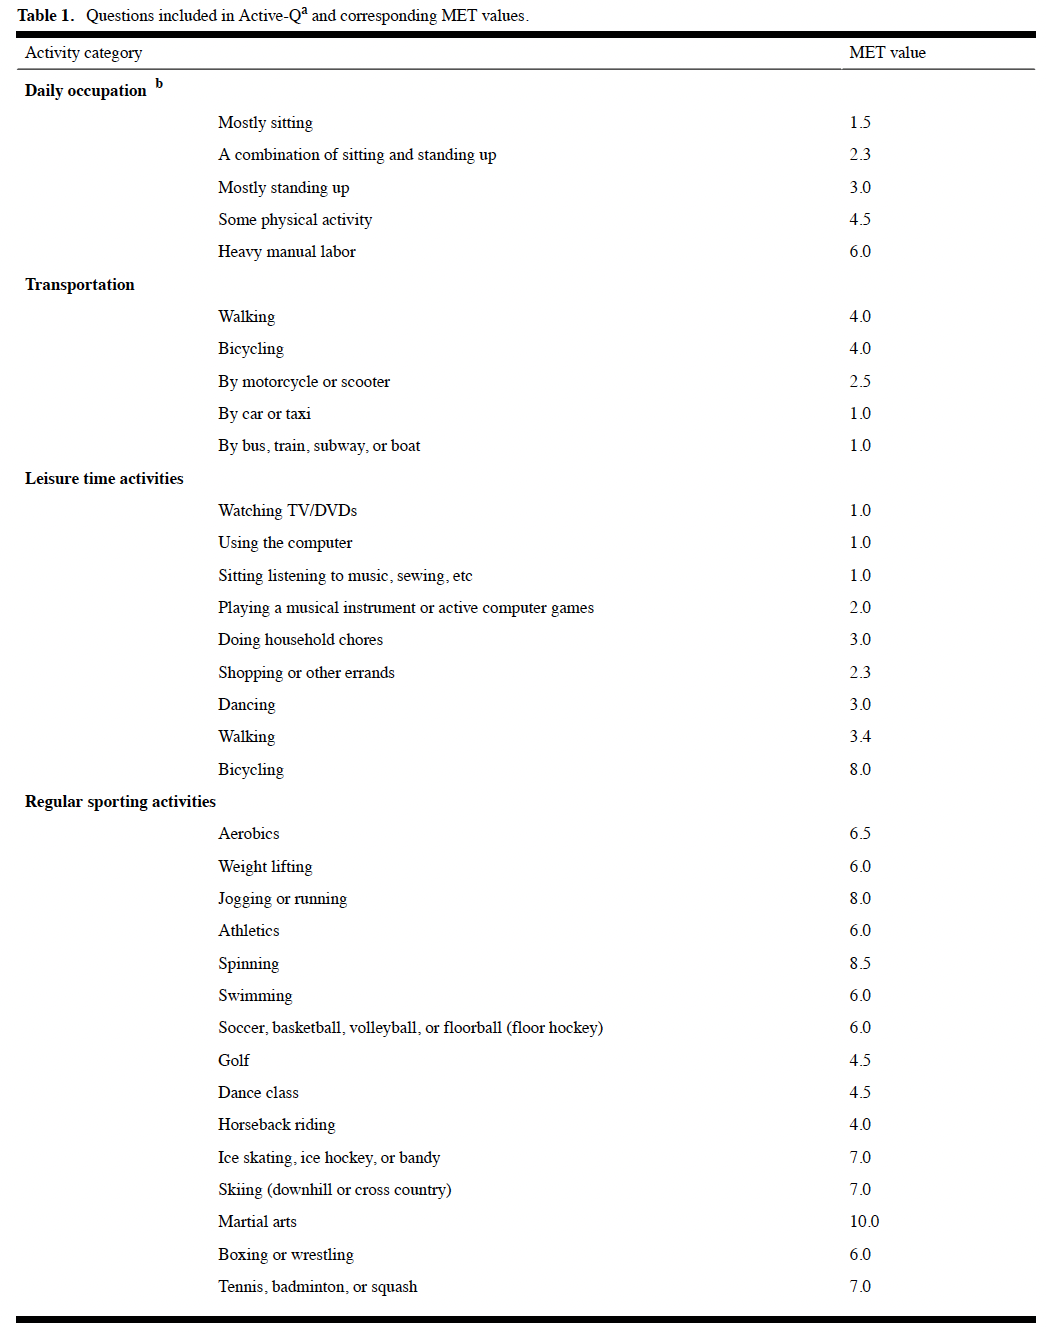
\includegraphics[width=0.8\textwidth]{appendix/met_values.png}
    \caption{MET value labels \parencite{Bonn_2012}}
    \label{fig: met_values}
\end{figure}
\begin{figure}[ht]
    \centering
    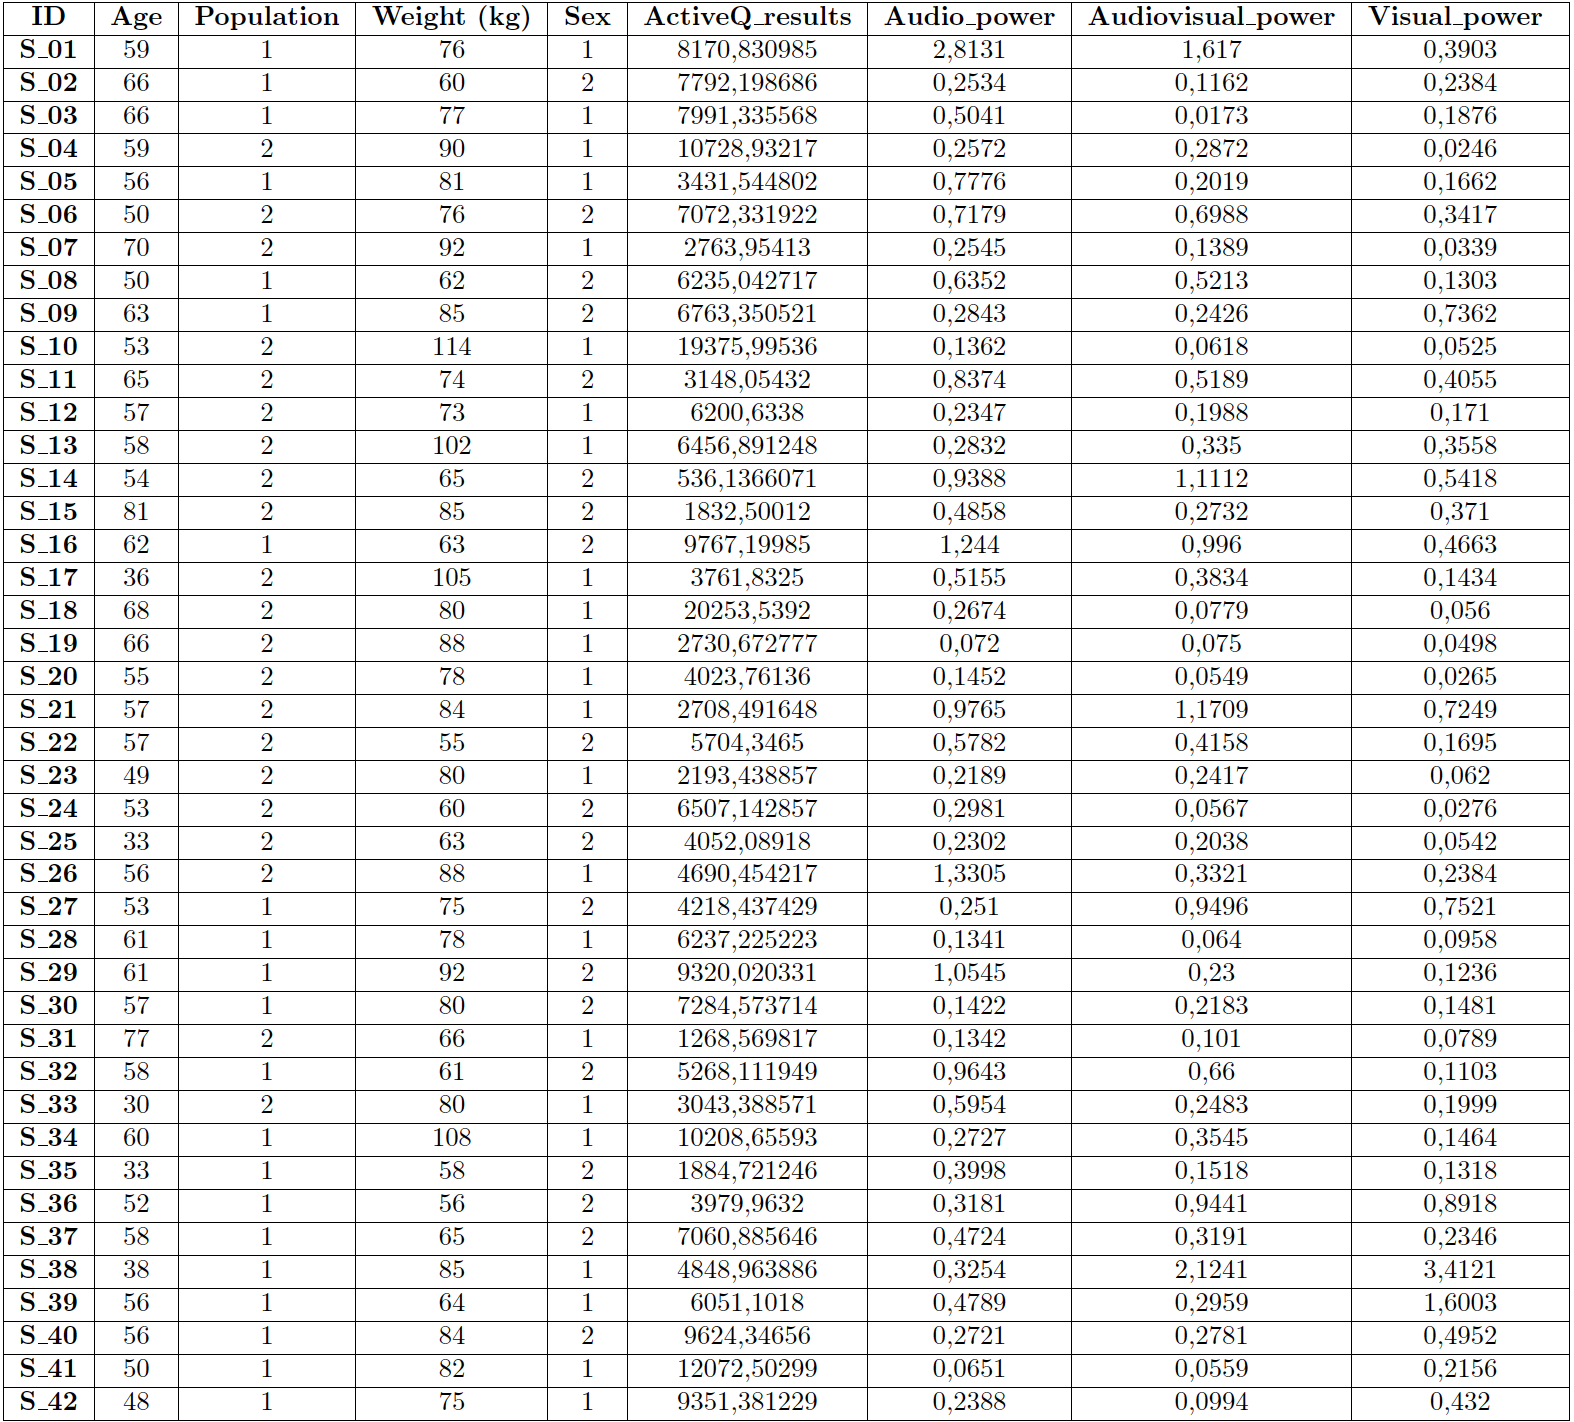
\includegraphics[width=0.95\textwidth]{appendix/database.png}
    \caption{Participants database with results}
    \label{fig: database}
\end{figure}
\begin{figure}[ht]
    \centering
    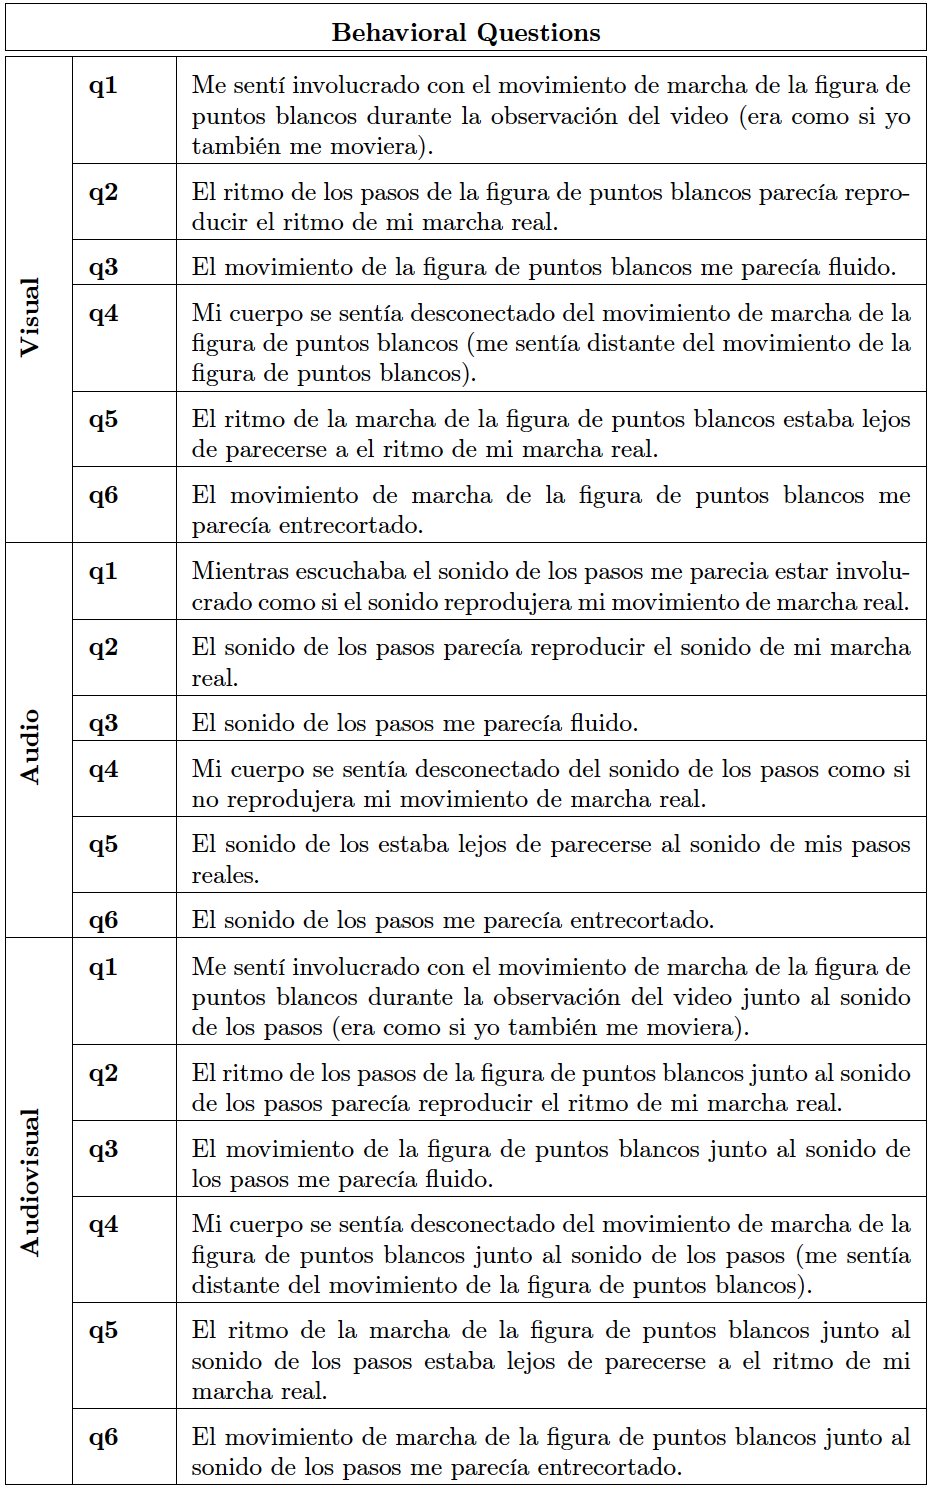
\includegraphics[width=0.70\textwidth]{appendix/questions.png}
    \caption{Participants database with results}
    \label{fig: Behavioral questions}
\end{figure}

\clearpage
\section*{Results}
\subsection*{Activity power spectrum}
\begin{figure}[H]
    \centering
    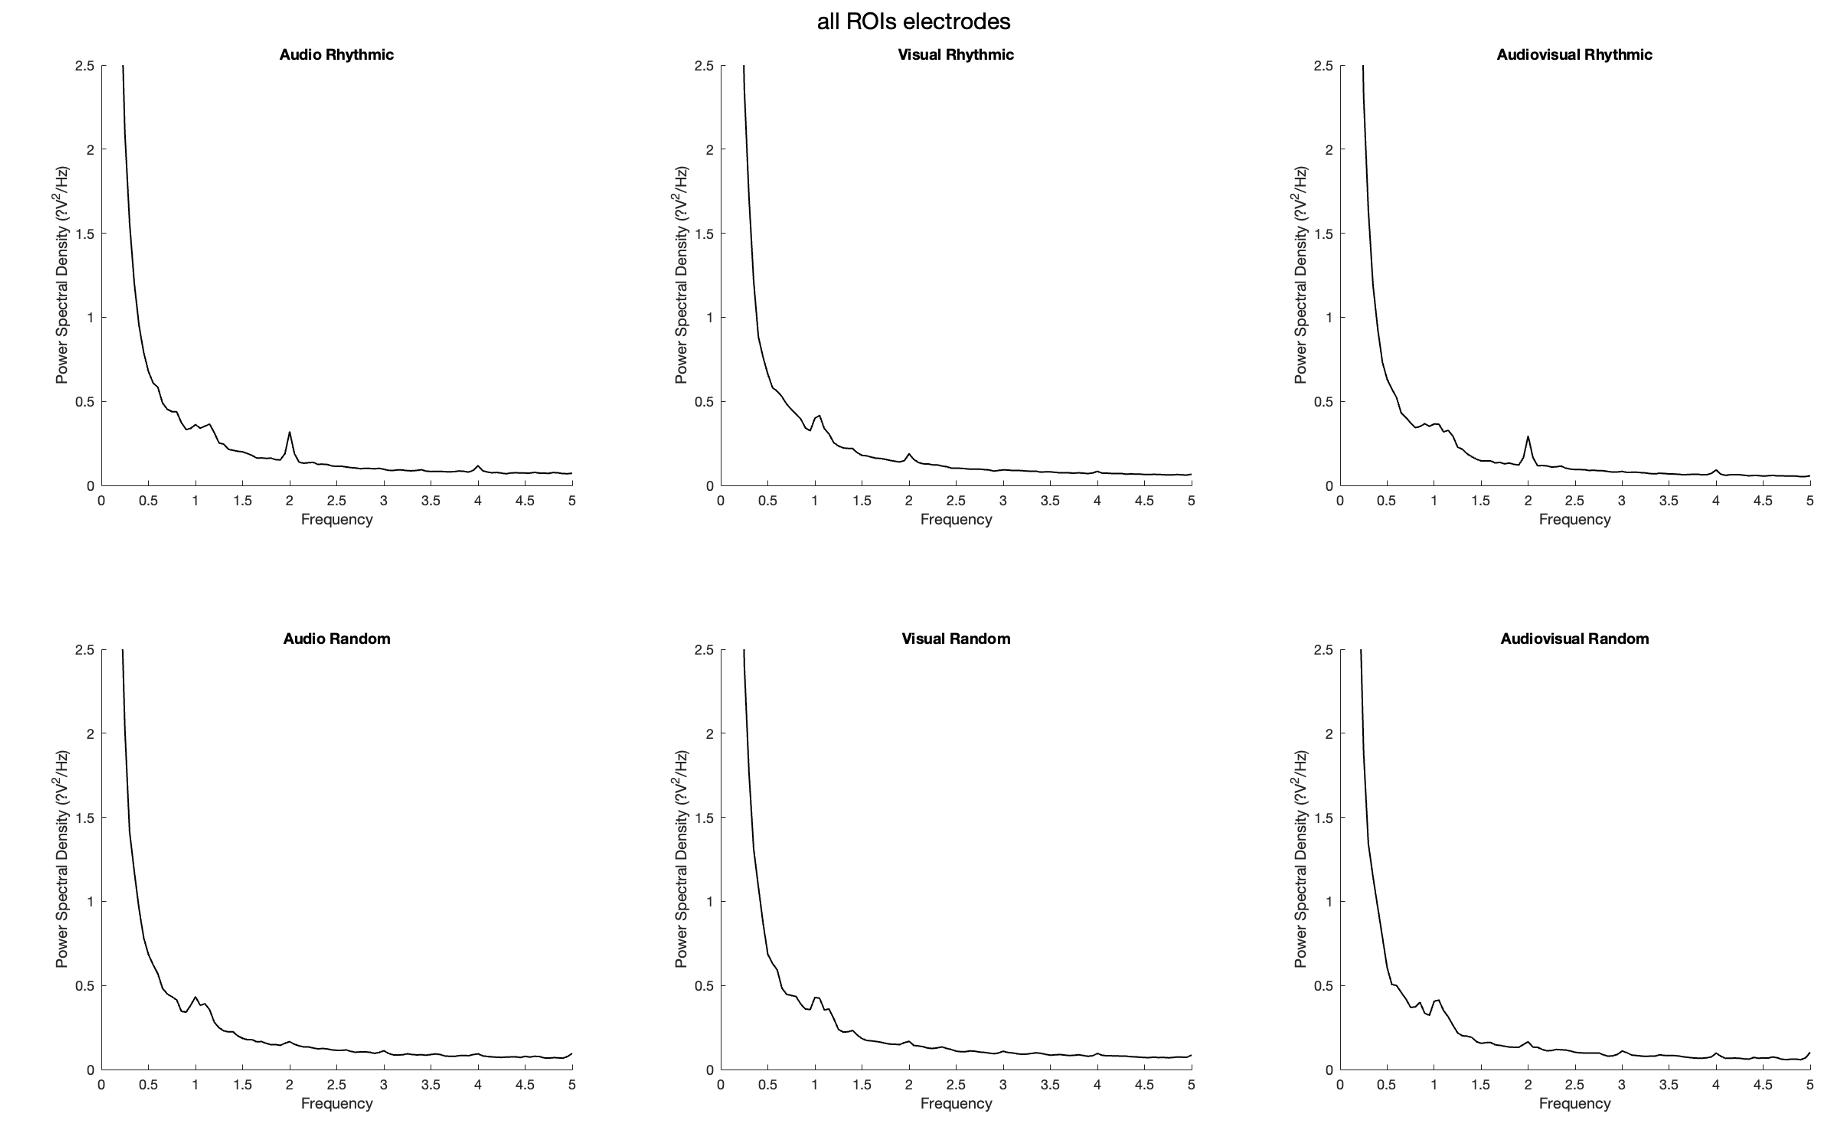
\includegraphics[width=0.85\textwidth]{healthy_images/allROI_graph.png}
    \caption{Activity peaks taking all the ROIs in consideration}
    \label{fig: allROI}
\end{figure}
\begin{figure}[H]
    \centering
    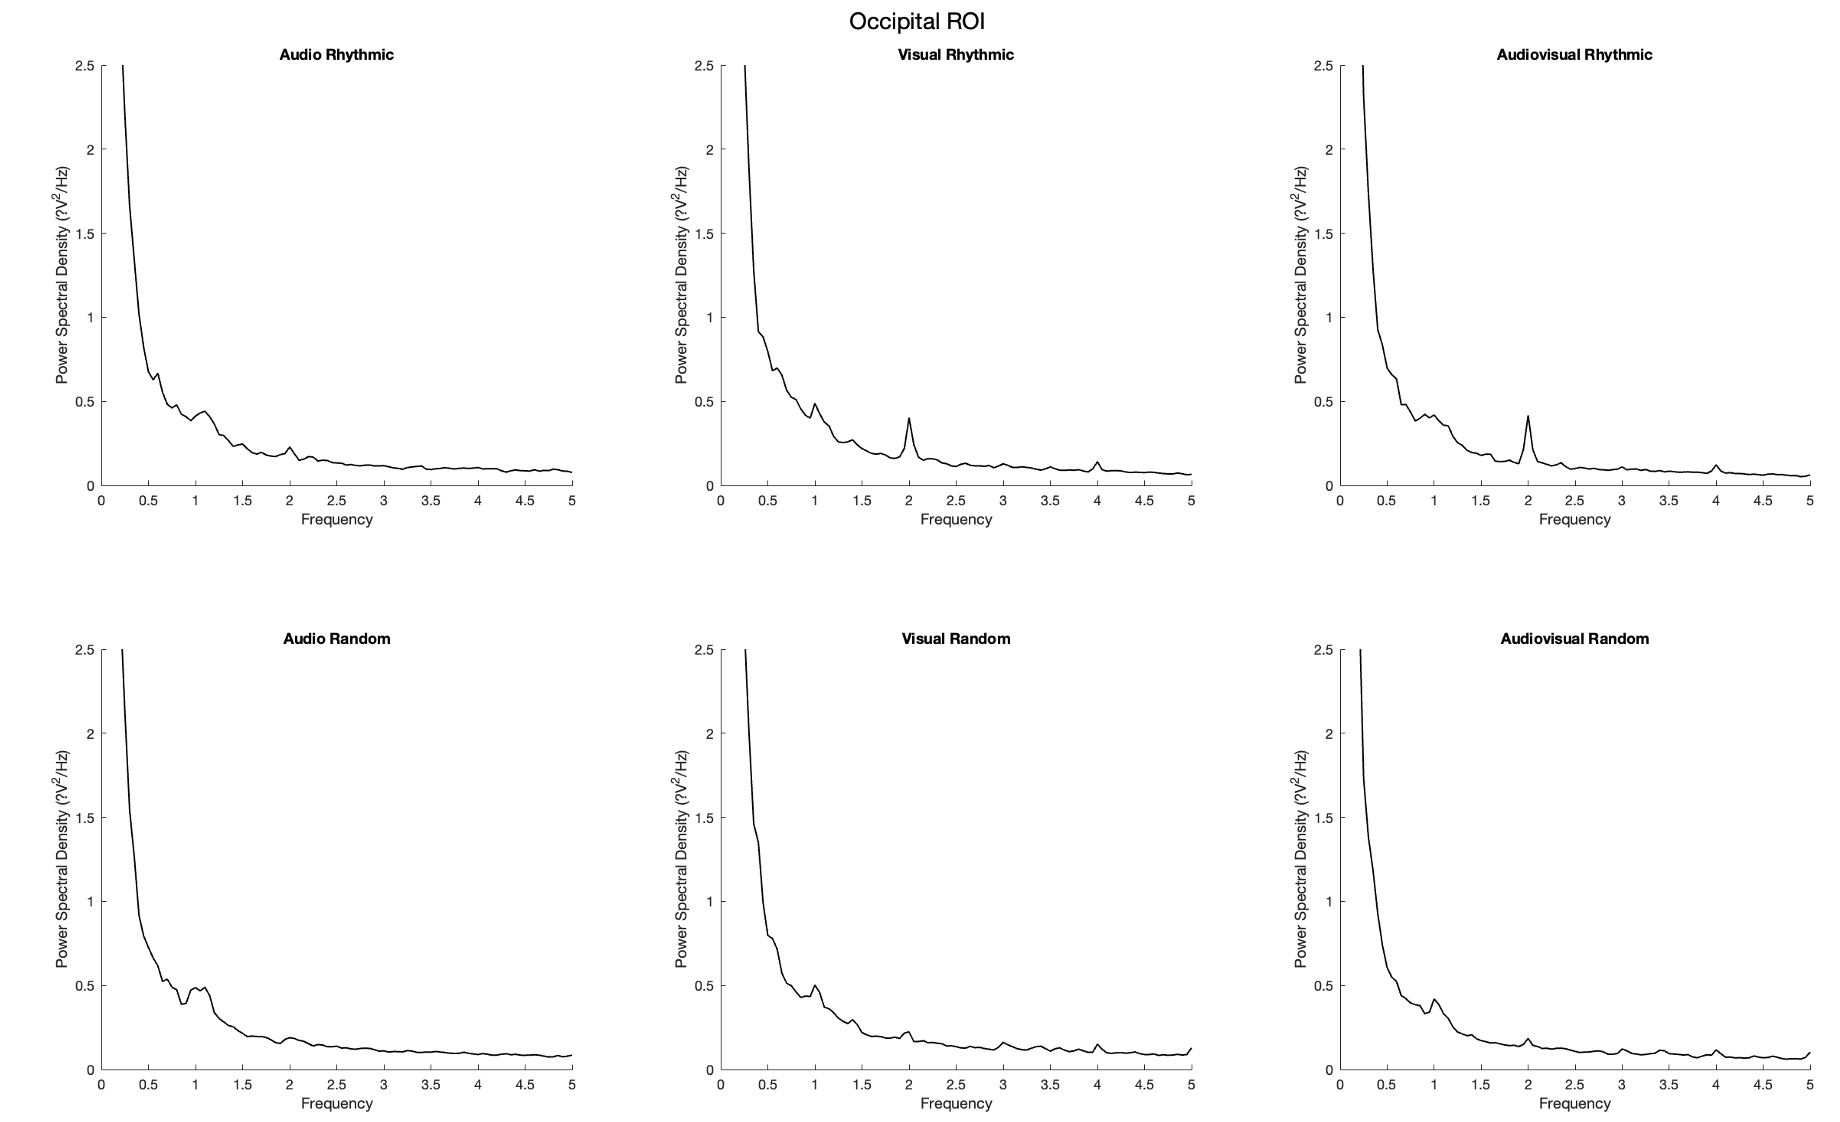
\includegraphics[width=0.85\textwidth]{healthy_images/occipitalROI_graph.png}
    \caption{Activity peak in the occipital ROI}
    \label{fig: occipital ROI}
\end{figure}
\begin{figure}[H]
    \centering
    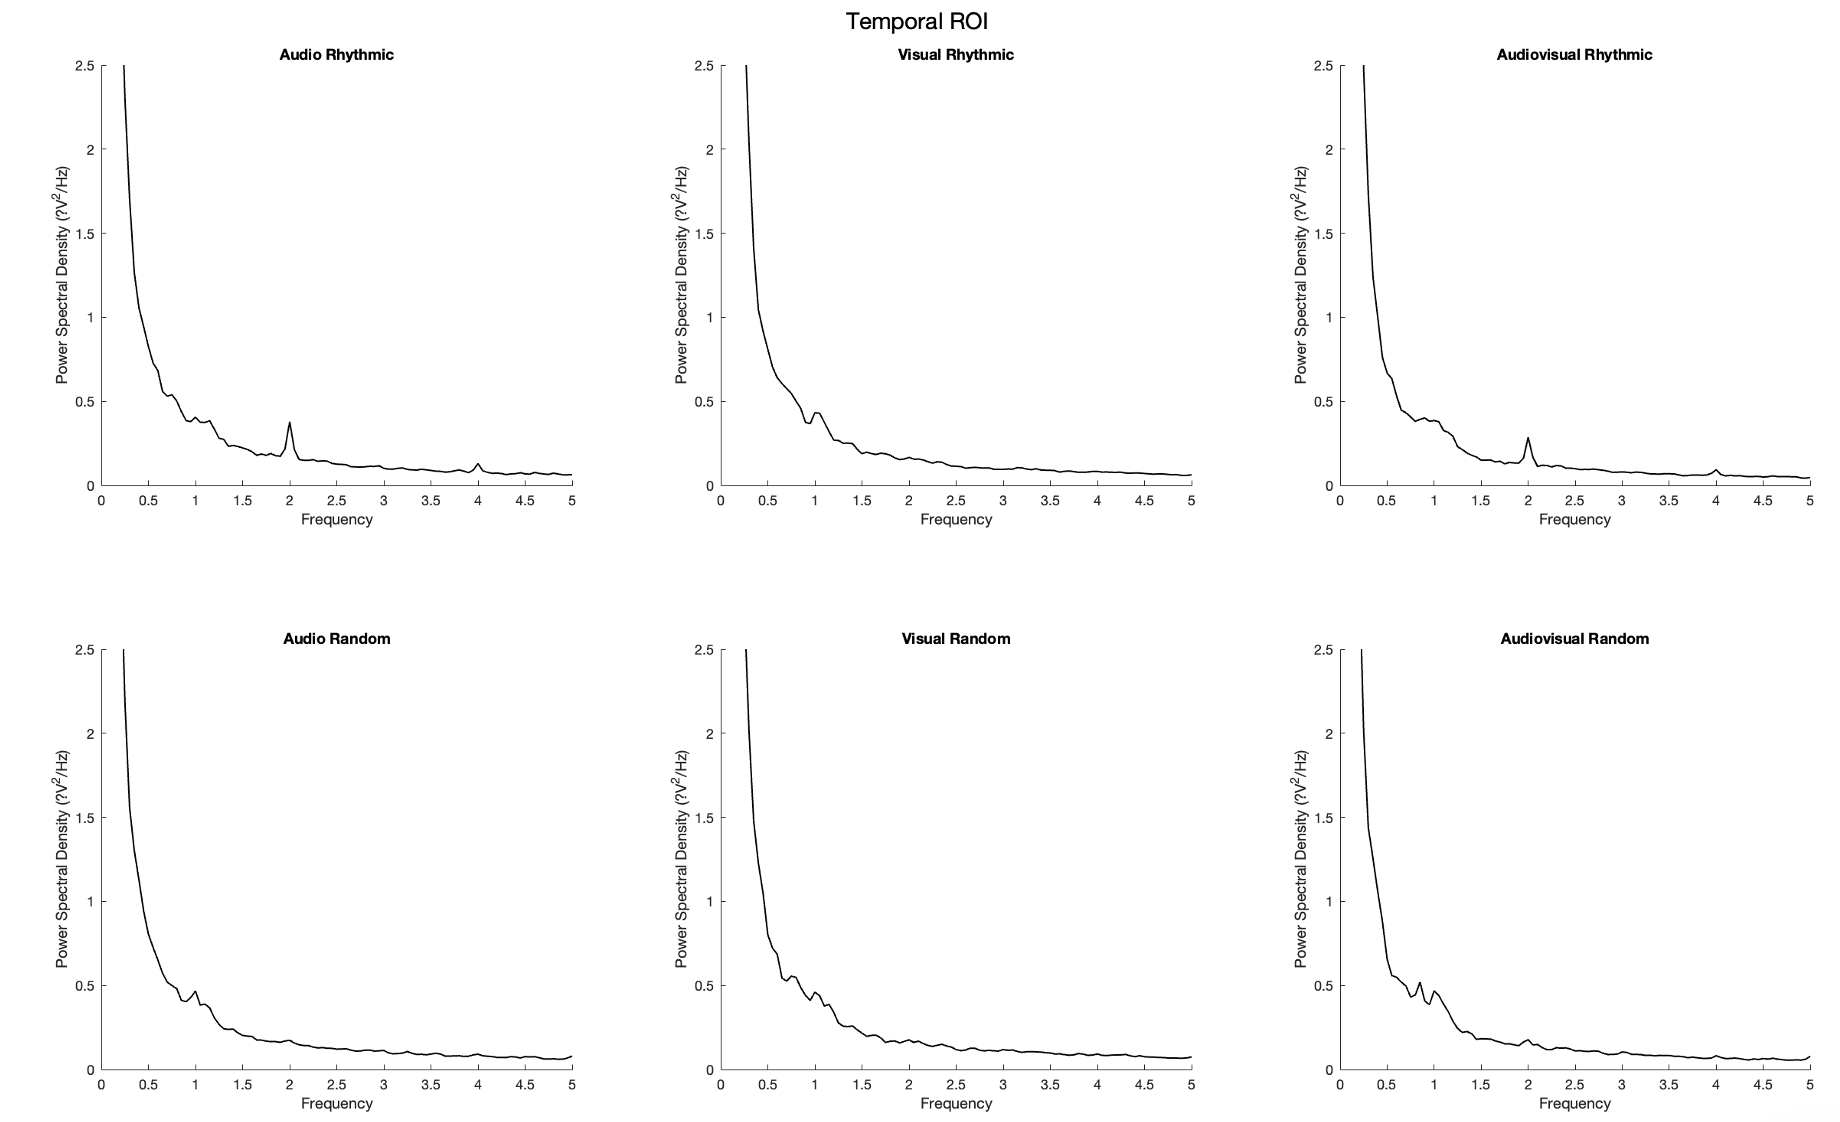
\includegraphics[width=0.85\textwidth]{healthy_images/temporalROI_graph.png}
    \caption{Activity peak in the temporal ROI}
    \label{fig: temporal ROI}
\end{figure}
\begin{figure}[H]
    \centering
    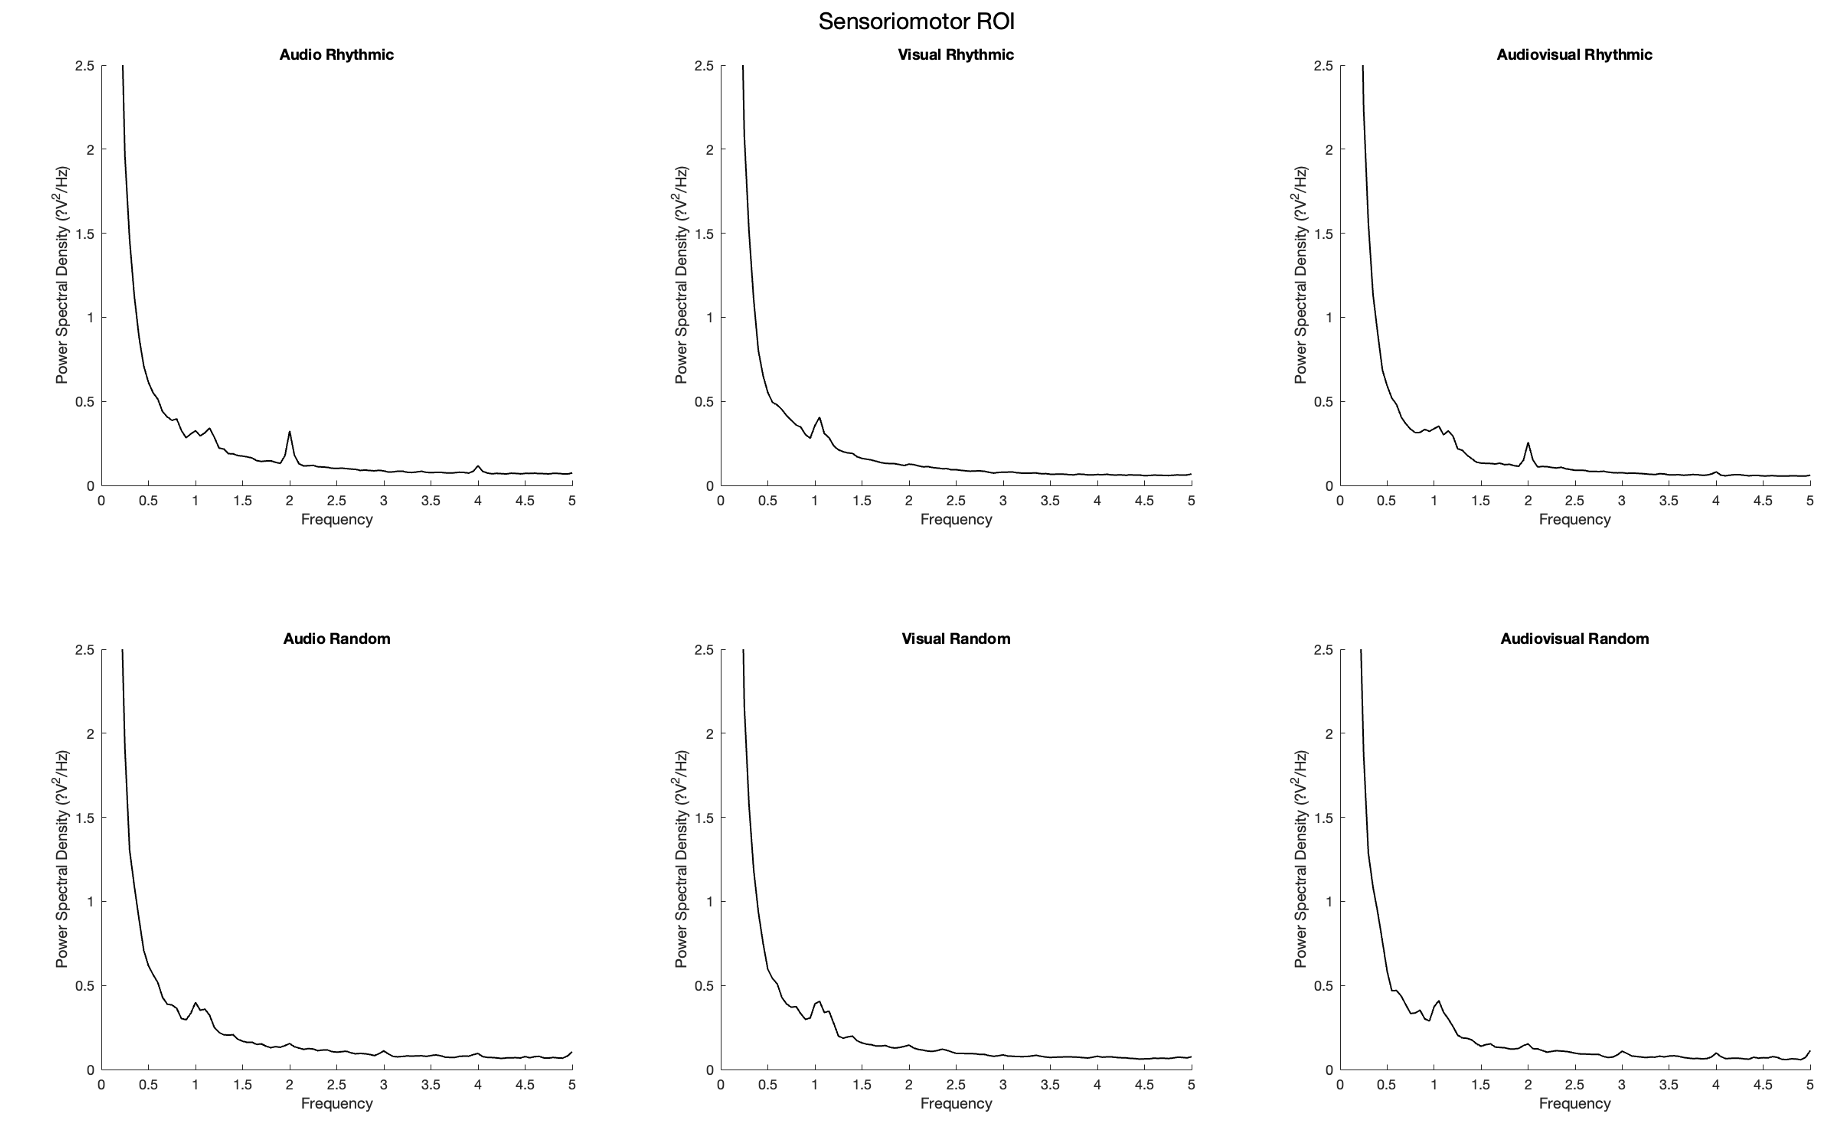
\includegraphics[width=0.85\textwidth]{healthy_images/sensorimotorROI_graph.png}
    \caption{Activity peak in the sensorimotor ROI}
    \label{fig: sensorimotor ROI} 
\end{figure} 

\clearpage
\subsection*{Topographies}
\begin{figure}[htbp]
    \centering
    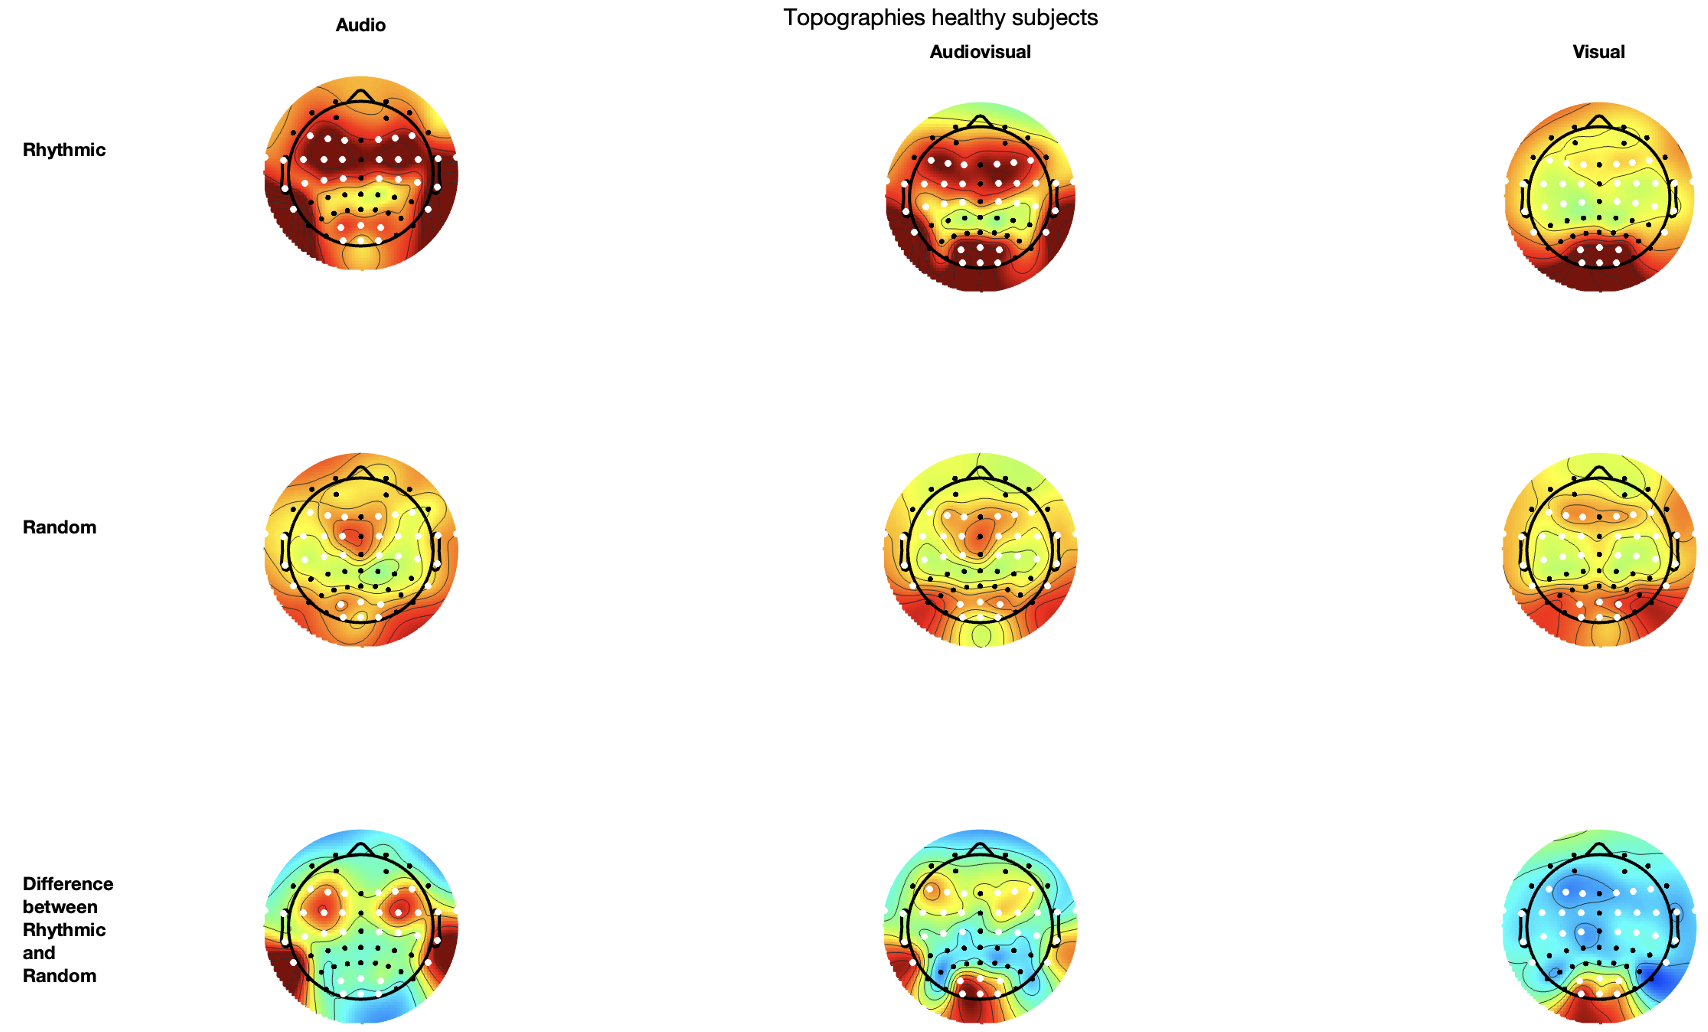
\includegraphics[width=0.85\textwidth]{healthy_images/topo.png}
    \caption{Topographies related to the activity in the control group}
    \label{fig: topographies control group}
\end{figure}
\begin{figure}[htbp]
    \centering
    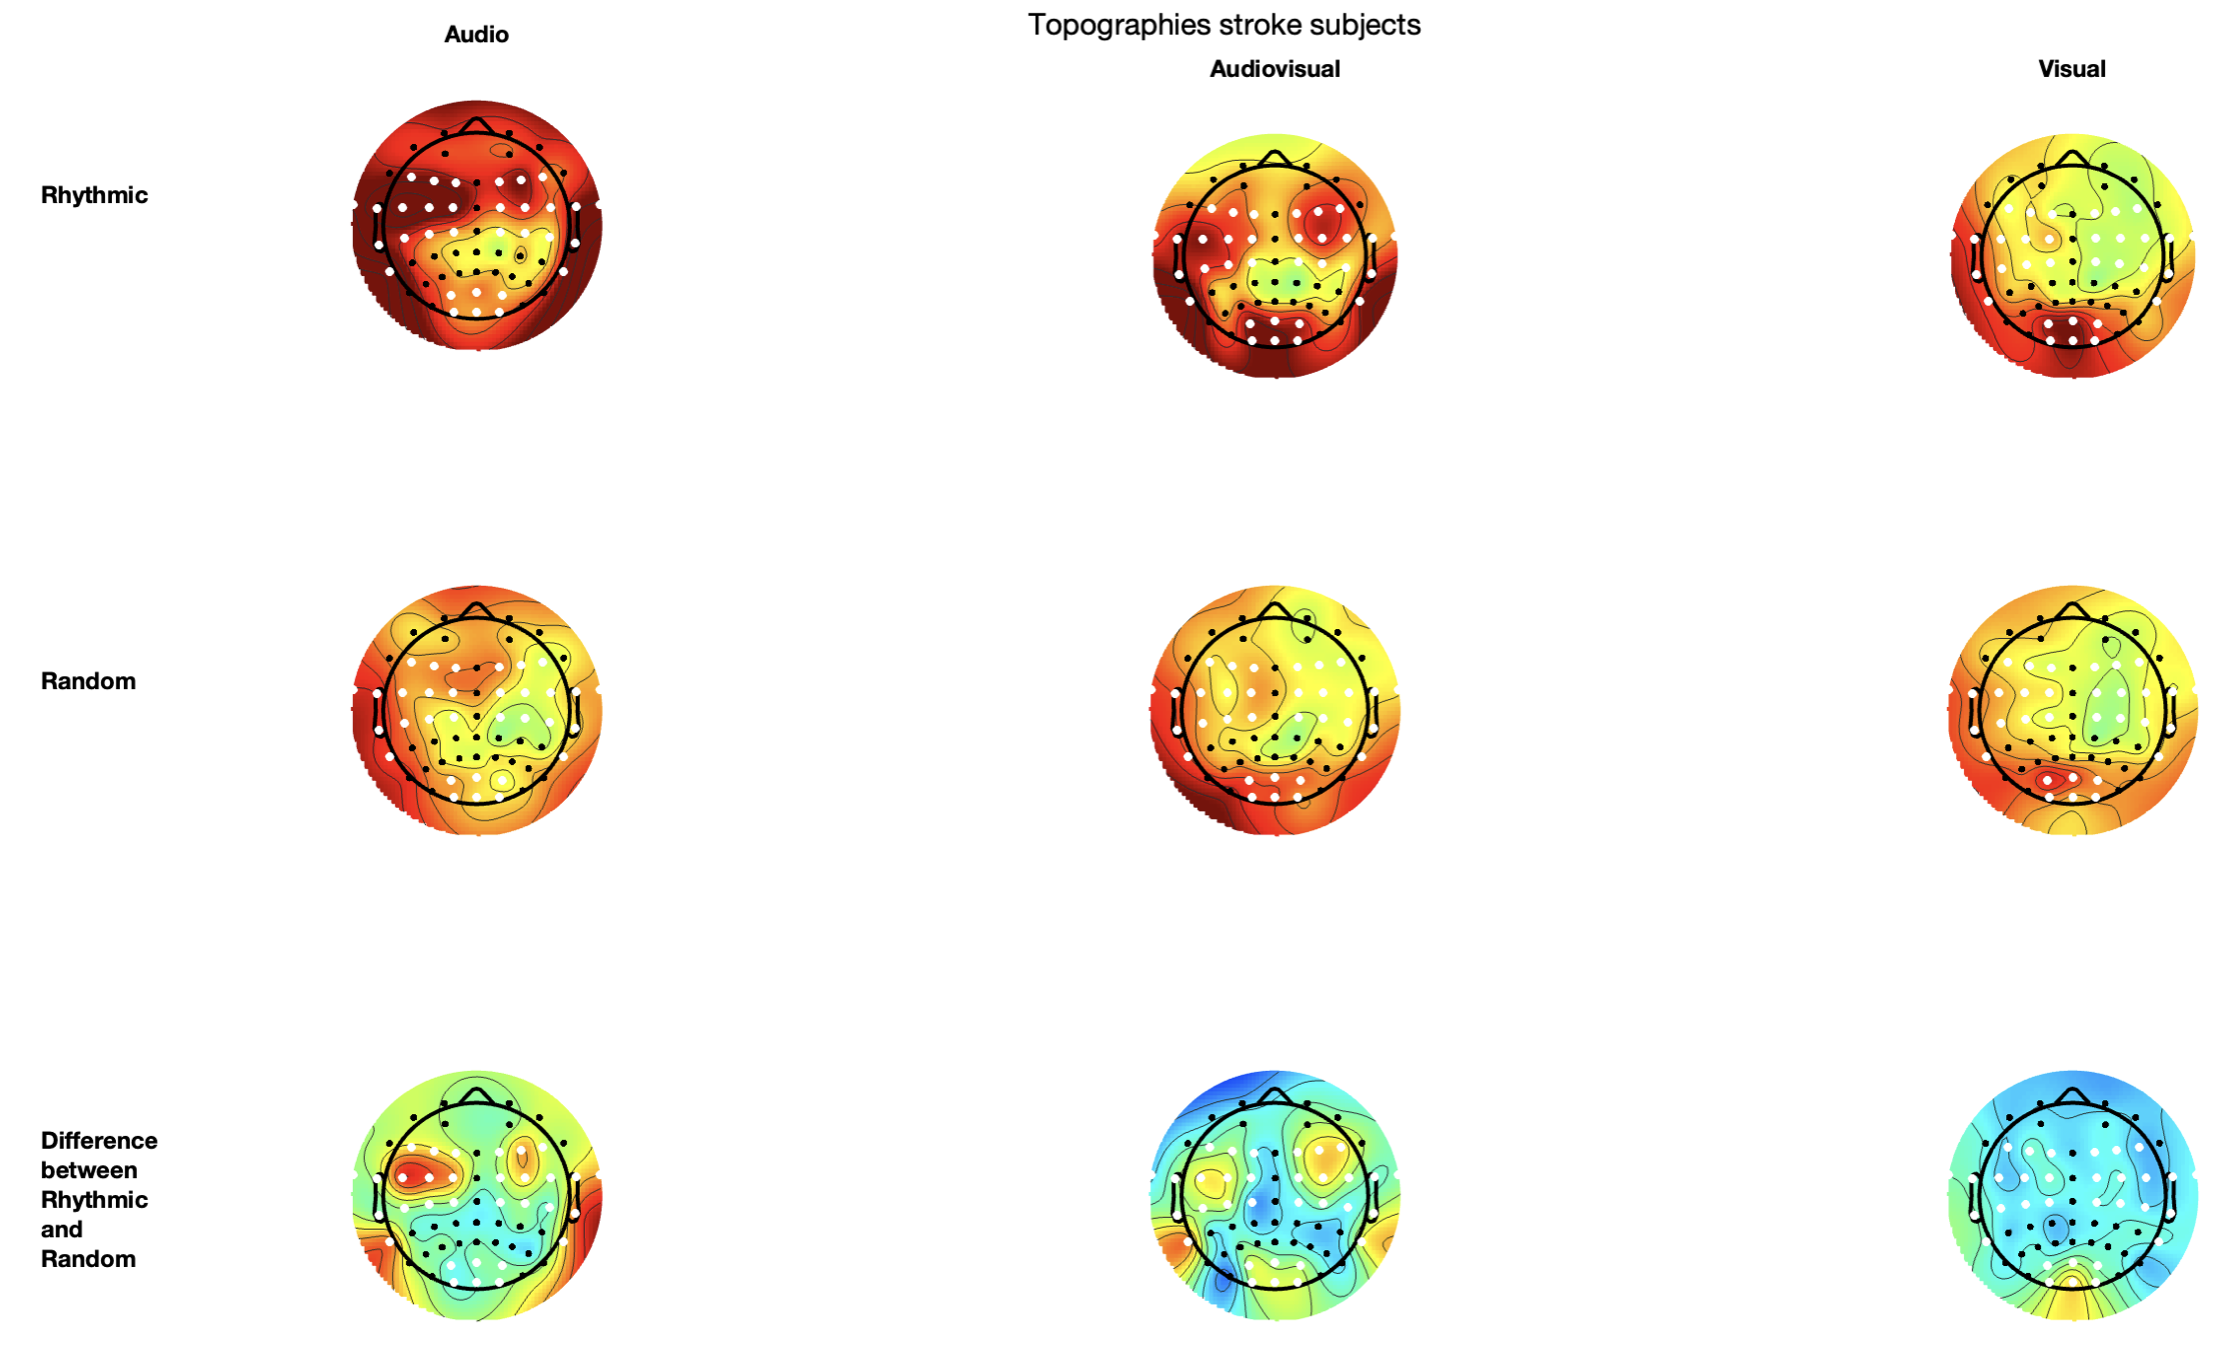
\includegraphics[width=0.85\textwidth]{stroke_images/topographies.png}
    \caption{Topographies related to the activity in stroke population}
    \label{fig: topographies stroke group}
\end{figure}
\begin{figure}[htbp]
    \centering
    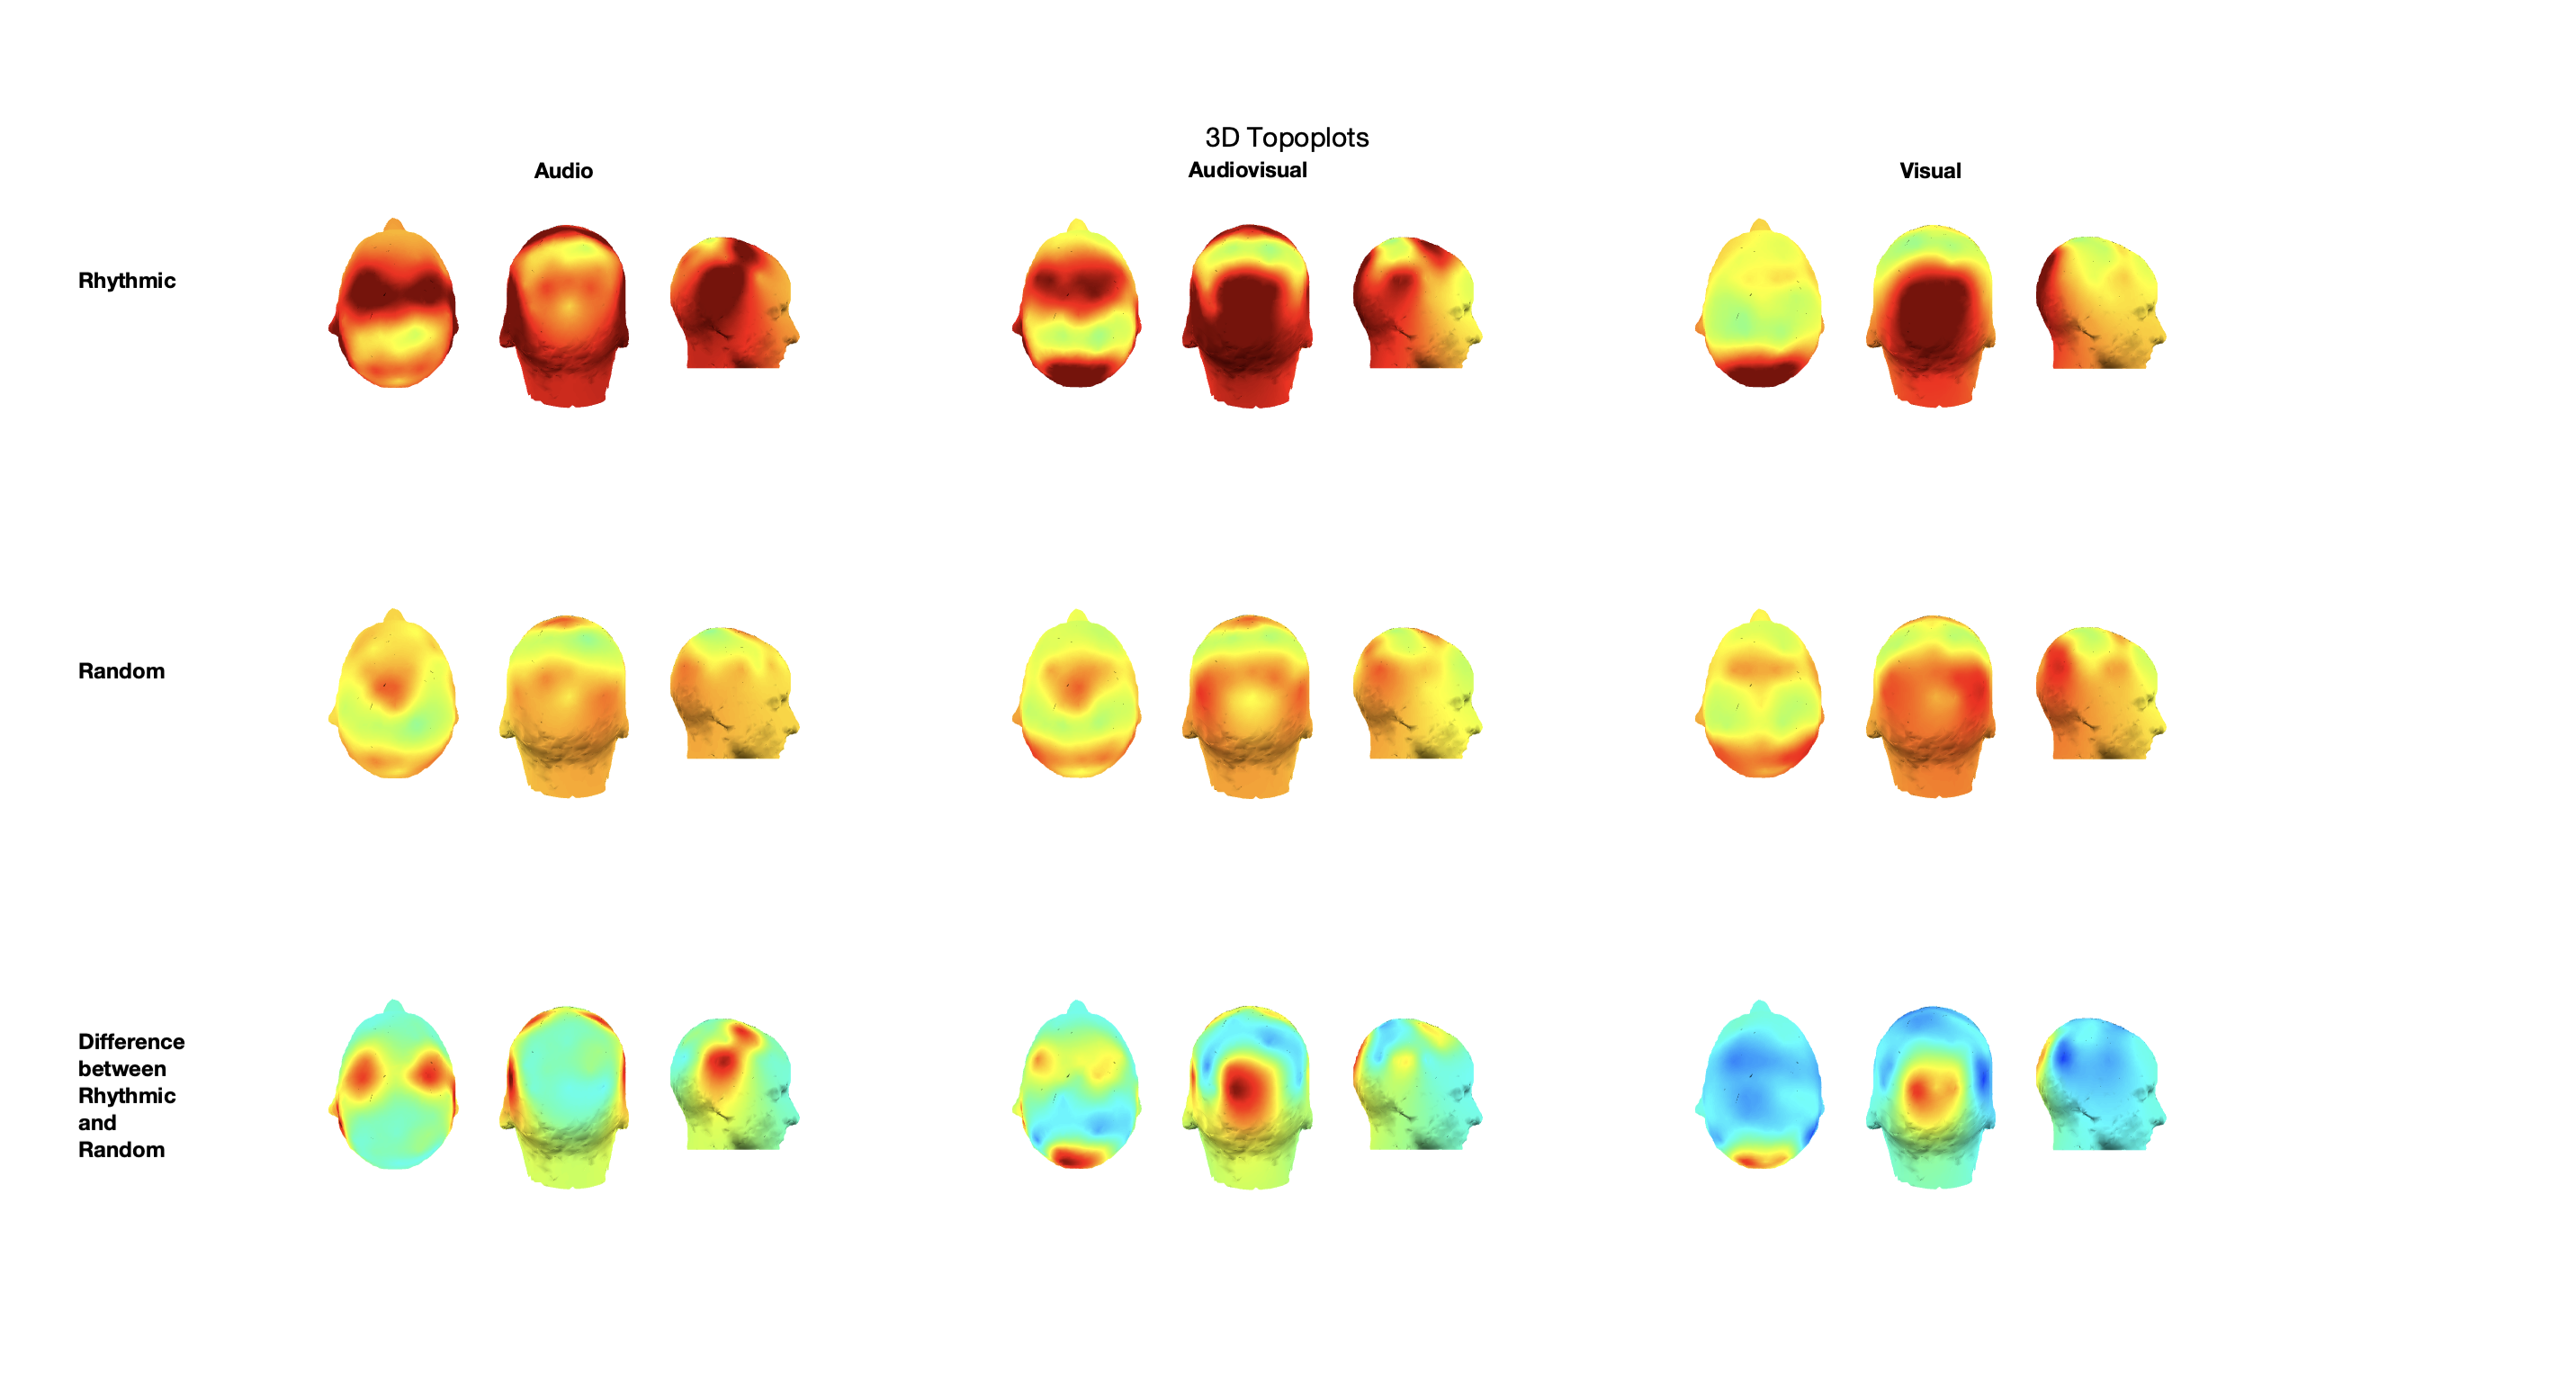
\includegraphics[width=0.85\textwidth]{healthy_images/3d_topo.png}
    \caption{3D topographies related to the activity in the control group}
    \label{fig: 3D topographies control group}   
\end{figure} 
\begin{figure}[htbp]
    \centering
    \includegraphics[width=0.85\textwidth]{stroke_images/3d_topographies.png}
    \caption{3D topographies related to the activity in stroke population}
    \label{fig: 3D topographies stroke group}   
\end{figure} 

\clearpage
\subsection*{Bar plots related to behavioral questions}
% \subsubsection*{Total population}
% \begin{figure}[H]
%     \centering
%     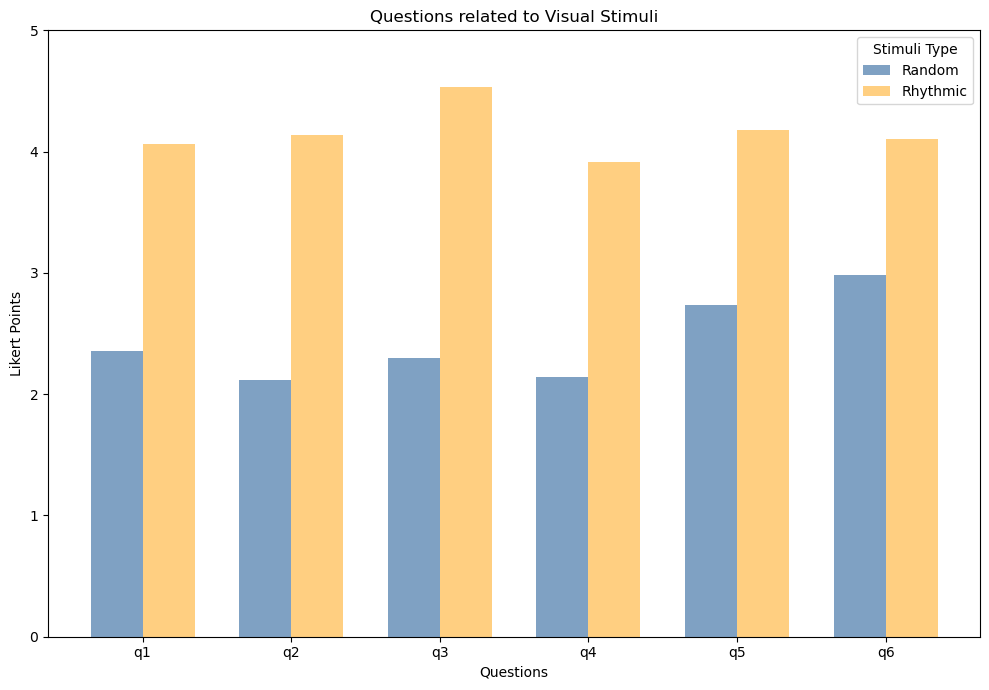
\includegraphics[width=0.85\textwidth]{bar_plots/bar_visual_t.png}
%     \caption{Results of behavioral question in the visual condition in the total population}
%     \label{fig: bar_visual_Total} 
% \end{figure}
% \begin{figure}[H]
%     \centering
%     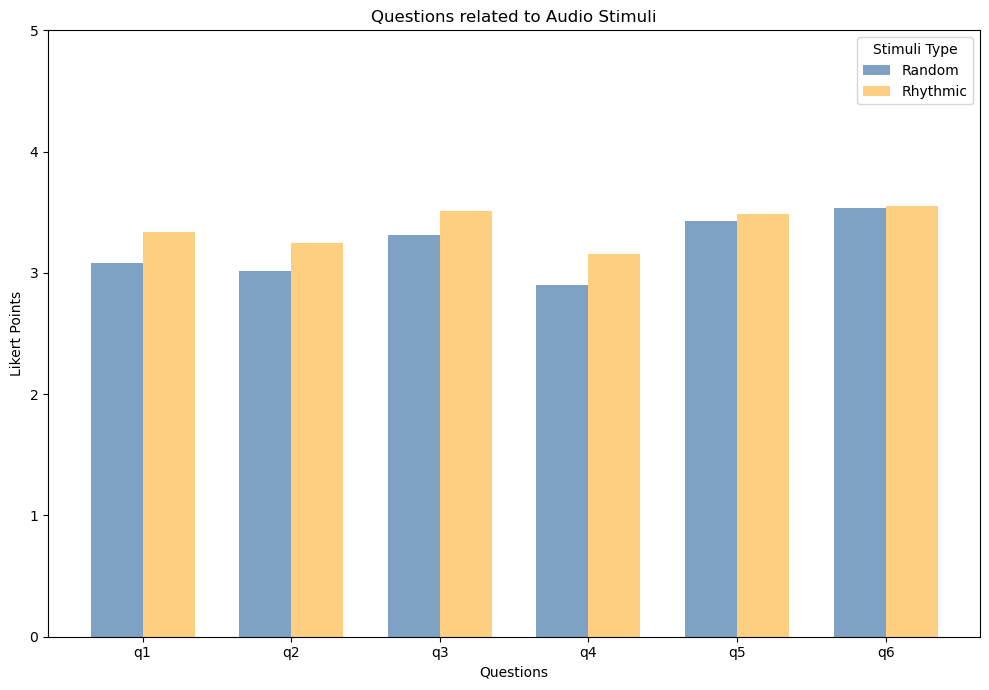
\includegraphics[width=0.85\textwidth]{bar_plots/bar_audio_t.png}
%     \caption{Results of behavioral question in the audio condition in the total population}
%     \label{fig: bar_audio_Total} 
% \end{figure} 
% \begin{figure}[H]
%     \centering
%     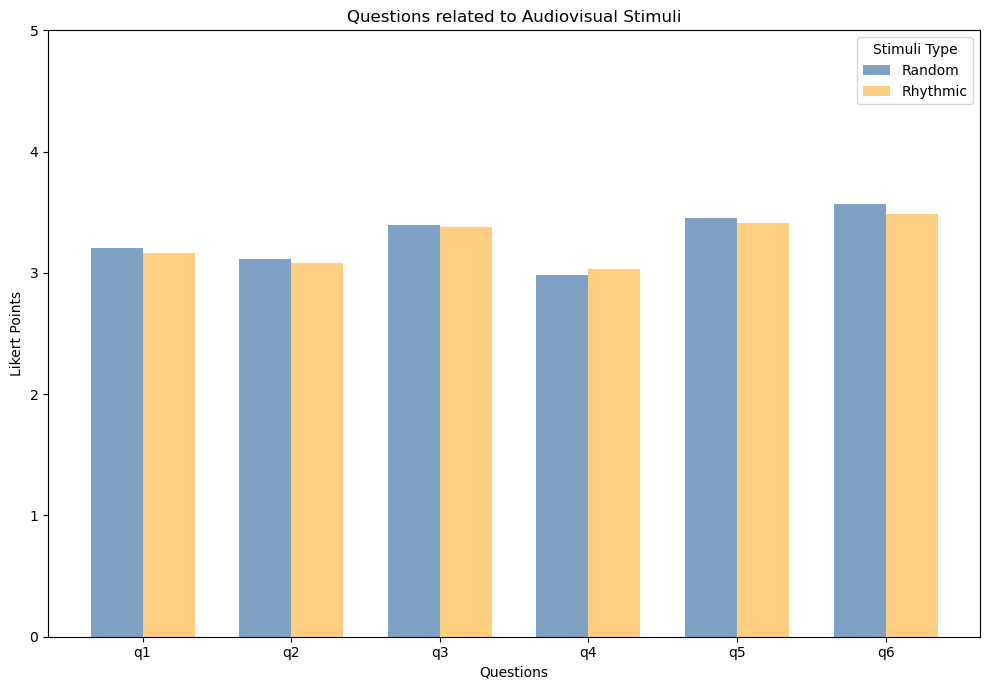
\includegraphics[width=0.85\textwidth]{bar_plots/bar_audiovisual_t.png}
%     \caption{Results of behavioral question in the audiovisual condition in the total population}
%     \label{fig: bar_audiovisual_Total} 
% \end{figure}  
% \begin{figure}[H]
%     \centering
%     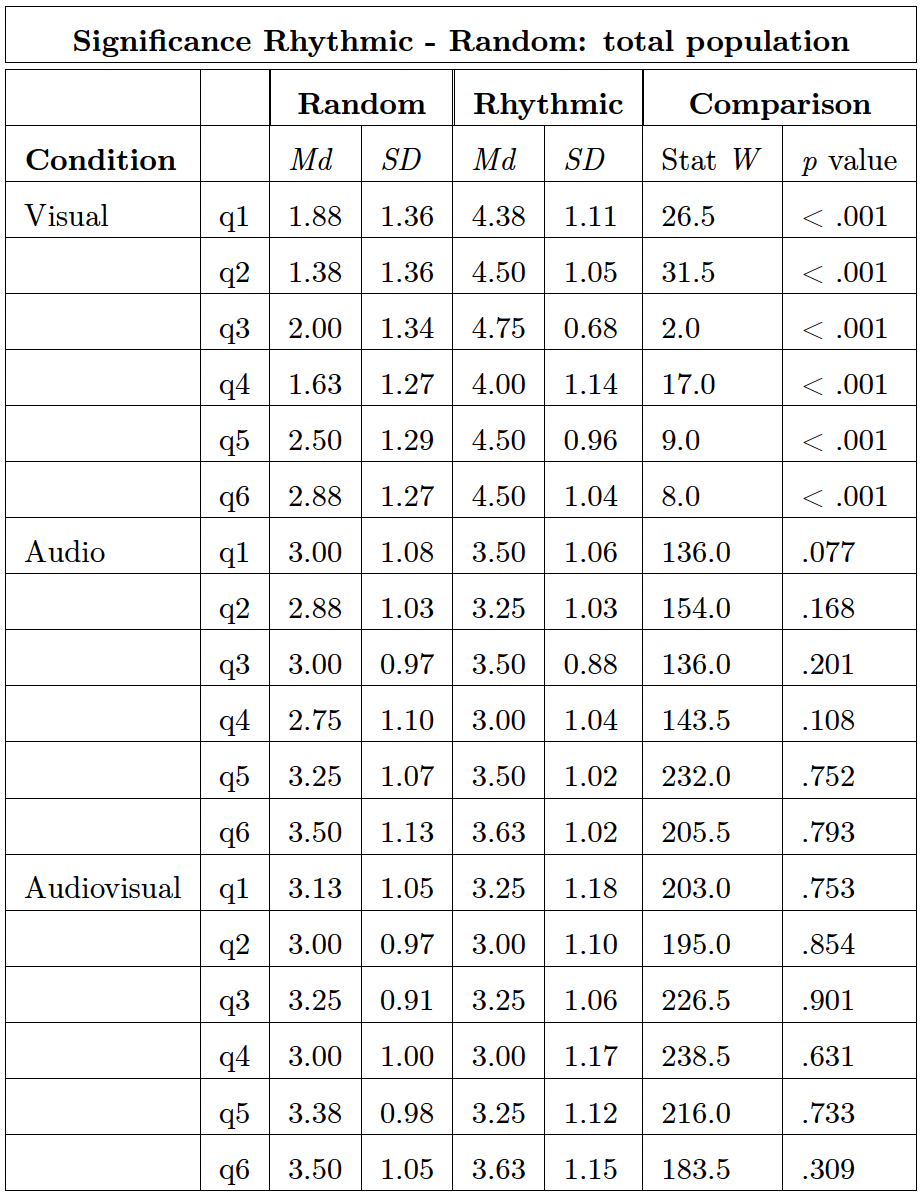
\includegraphics[width=0.55\textwidth]{significance_tables/total_pop.png}
%     \caption{Significance of the results of behavioral questions in the total population, using Wilcoxon Signed-Rank Test (\textit{W})}
%     \label{fig: significance_total_pop} 
% \end{figure} 

\subsubsection*{Control group}
\begin{figure}[H]
    \centering
    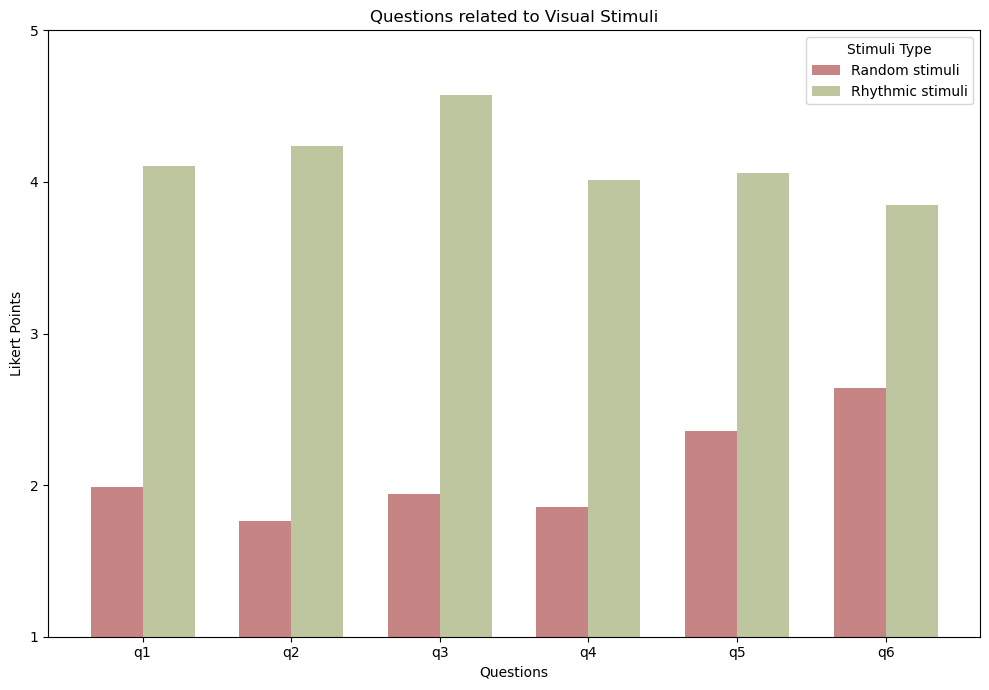
\includegraphics[width=0.85\textwidth]{bar_plots/bar_visual_h.png}
    \caption{Results of behavioral question in the visual condition in the control group}
    \label{fig: bar_control_Total} 
\end{figure} 
\begin{figure}[H]
    \centering
    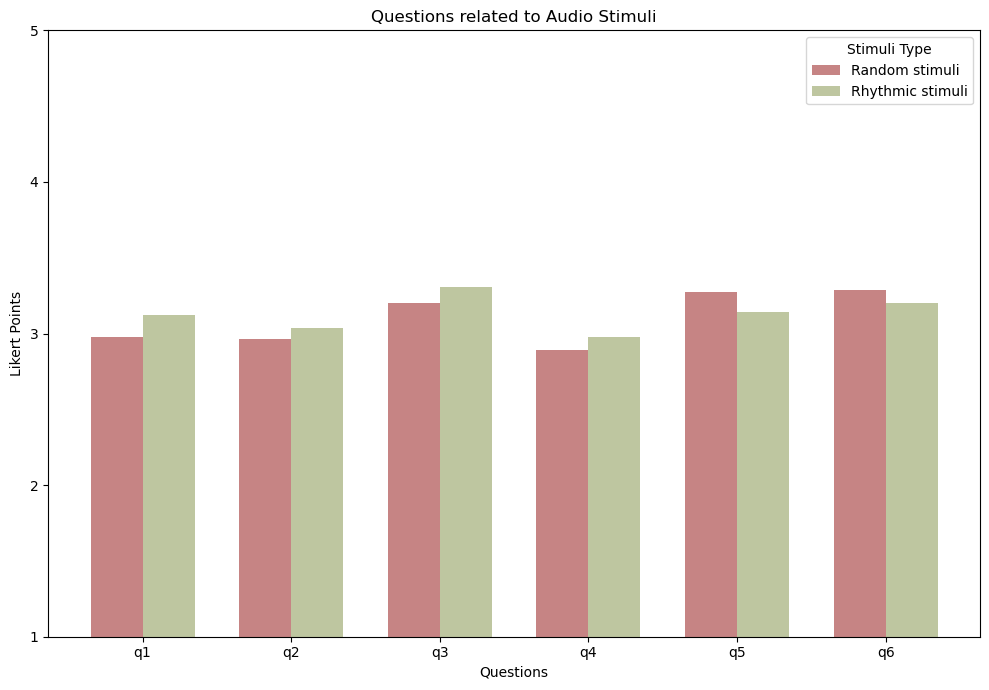
\includegraphics[width=0.85\textwidth]{bar_plots/bar_audio_h.png}
    \caption{Results of behavioral question in the audio condition in the control group}
    \label{fig: bar_audio_control} 
\end{figure} 
\begin{figure}[H]
    \centering
    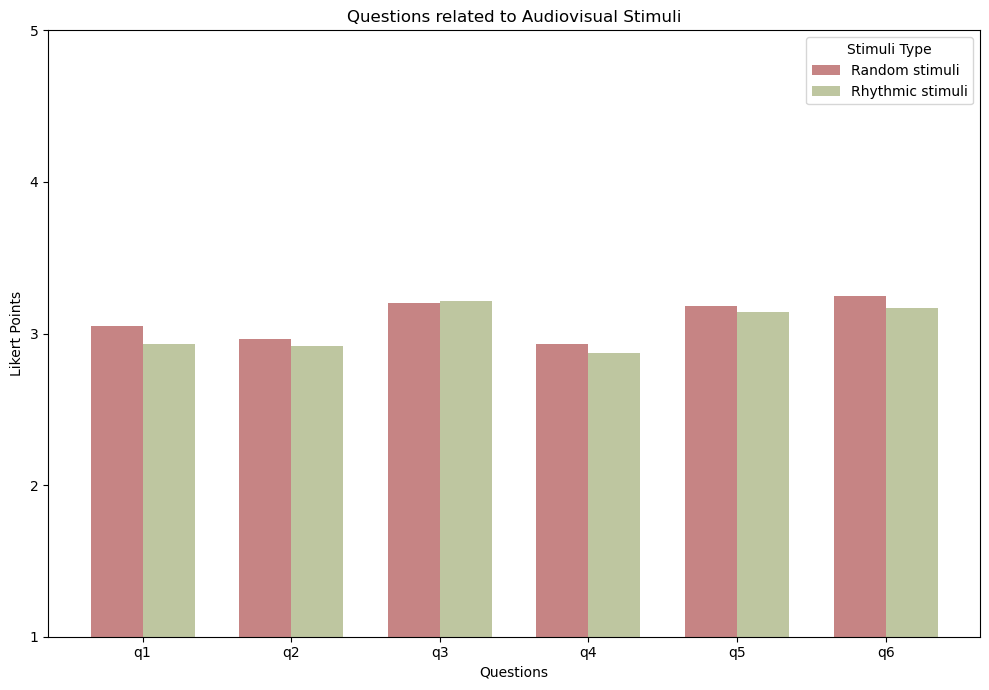
\includegraphics[width=0.85\textwidth]{bar_plots/bar_audiovisual_h.png}
    \caption{Results of behavioral question in the audiovisual condition in the control group}
    \label{fig: bar_audiovisual_control} 
\end{figure} 
\begin{figure}[H]
    \centering
    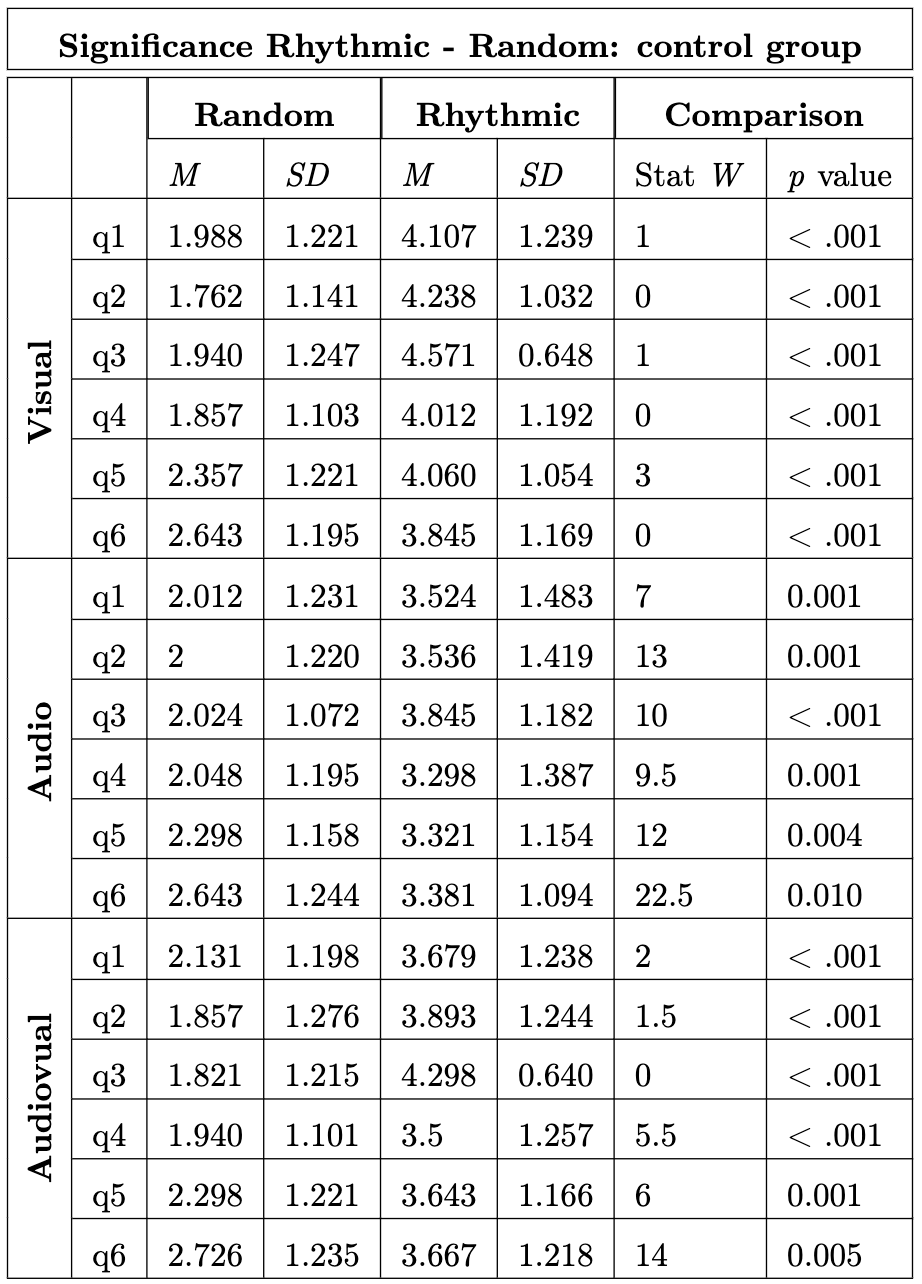
\includegraphics[width=0.55\textwidth]{significance_tables/control_group.png}
    \caption{Significance of the results of behavioral questions in the control group, using Wilcoxon Signed-Rank Test (\textit{W})}
    \label{fig: significance_control_pop} 
\end{figure} 

\subsubsection*{Stroke group}
\begin{figure}[H]
    \centering
    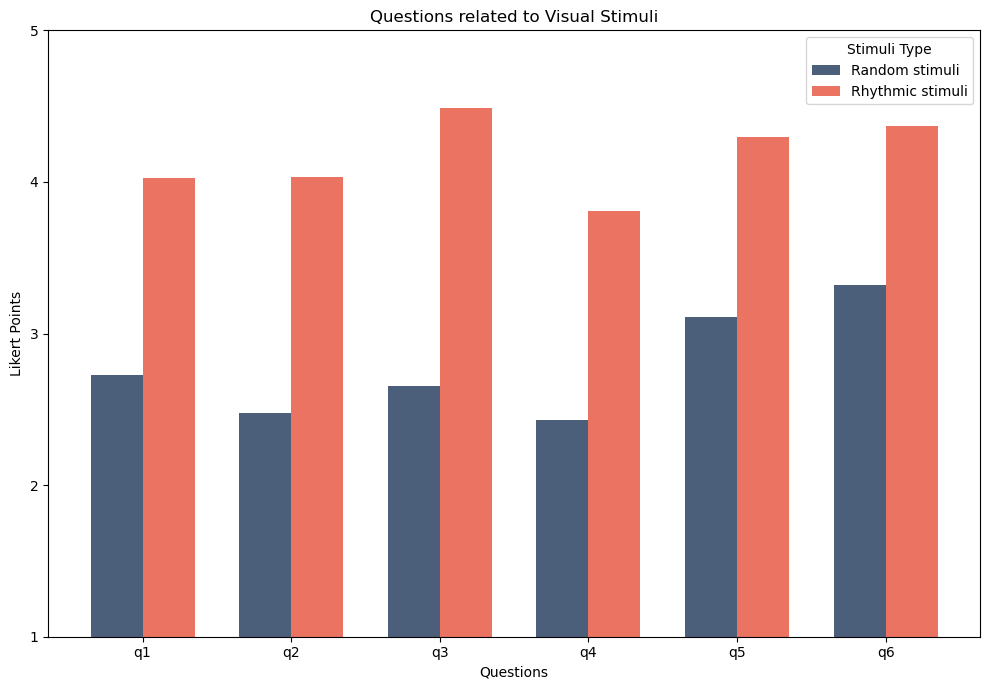
\includegraphics[width=0.85\textwidth]{bar_plots/bar_visual_s.png}
    \caption{Results of behavioral question in the visual condition in stroke population}
    \label{fig: bar_visual_stroke} 
\end{figure} 
\begin{figure}[H]
    \centering
    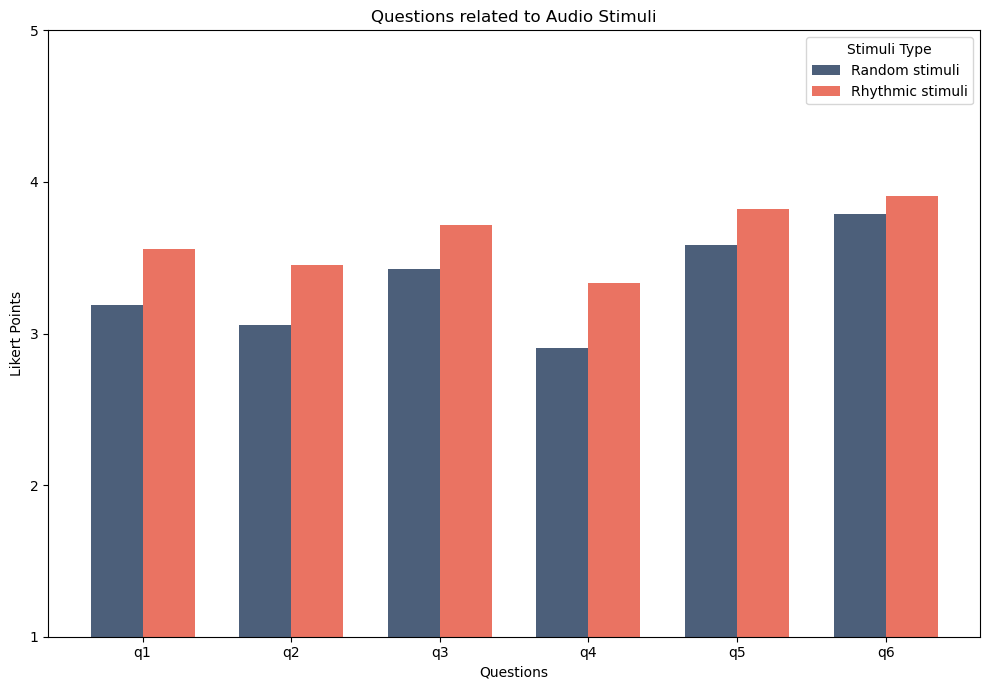
\includegraphics[width=0.85\textwidth]{bar_plots/bar_audio_s.png}
    \caption{Results of behavioral question in the audio condition in stroke population}
    \label{fig: bar_audio_stroke} 
\end{figure} 
\begin{figure}[H]
    \centering
    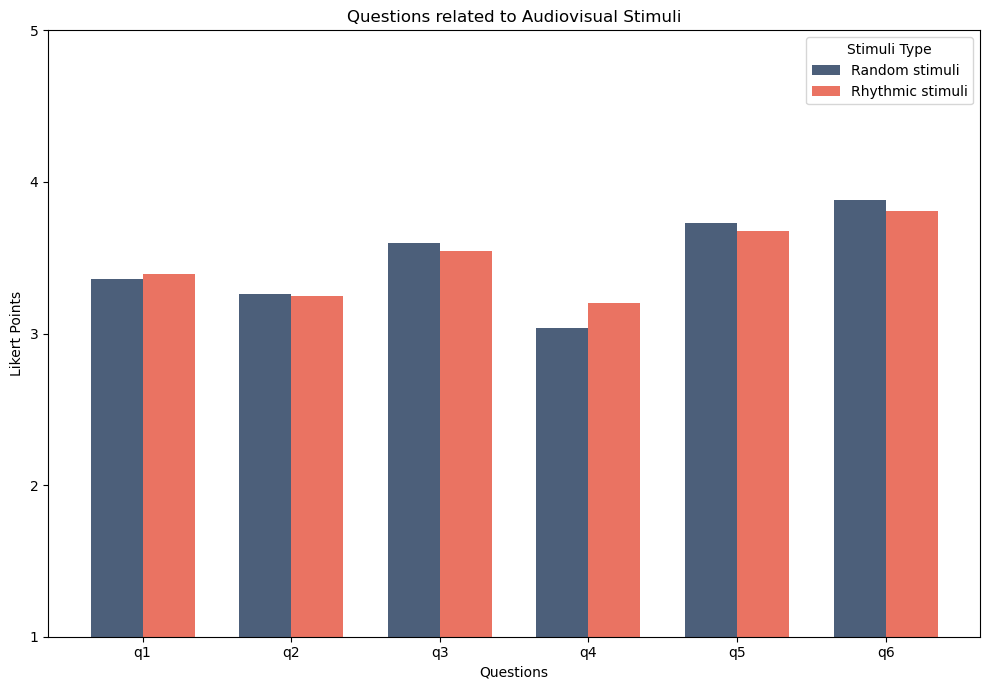
\includegraphics[width=0.85\textwidth]{bar_plots/bar_audvis_s.png}
    \caption{Results of behavioral question in the audiovisual condition in stroke population}
    \label{fig: bar_audiovisual_stroke} 
\end{figure} 
\begin{figure}[H]
    \centering
    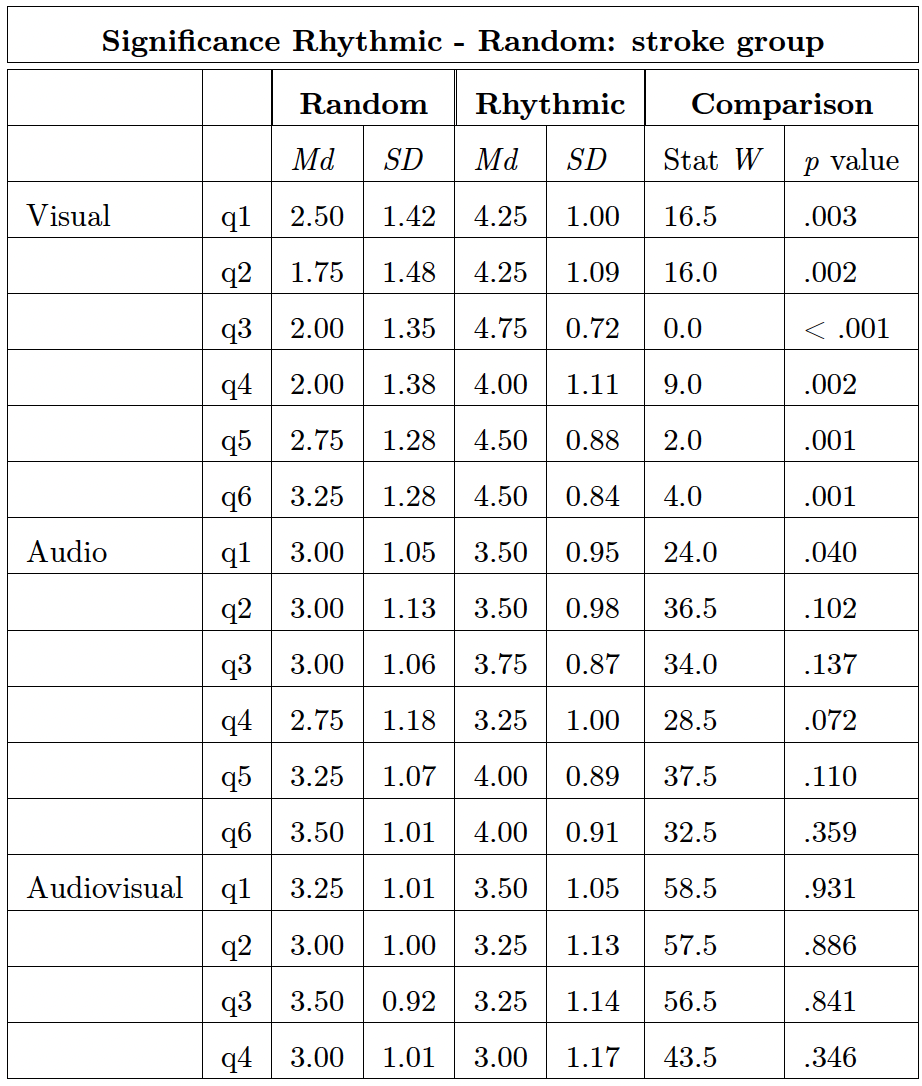
\includegraphics[width=0.60\textwidth]{significance_tables/stroke_group.png}
    \caption{Significance of the results of behavioral questions in the stroke group, using Wilcoxon Signed-Rank Test (\textit{W})}
    \label{fig: significance_stroke_pop} 
\end{figure} 

\subsubsection*{Total results mean}
% \begin{figure}[H]
%     \centering
%     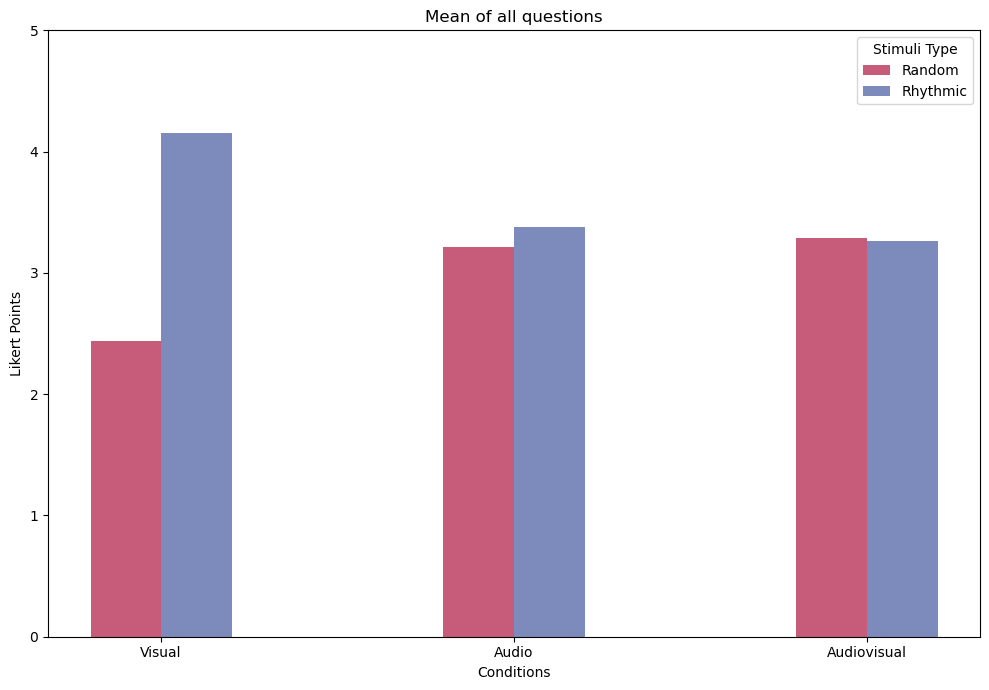
\includegraphics[width=0.85\textwidth]{bar_plots/mean_questions.png}
%     \caption{Mean of the results of all behavioral question in both population groups}
%     \label{fig: mean_total} 
% \end{figure} 
% \begin{figure}[H]
%     \centering
%     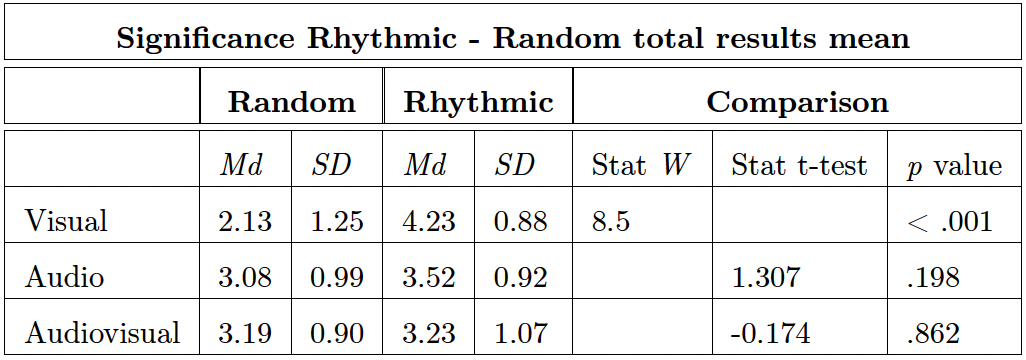
\includegraphics[width=0.65\textwidth]{significance_tables/tot_mean.png}
%     \caption{Significance of the results of all the behavioral questions, using Wilcoxon Signed-Rank Test (\textit{W}) or Paired Samples t-Test (\textit{t})}
%     \label{fig: significance_tot_mean} 
% \end{figure} 
% \clearpage
\begin{figure}[H]
    \centering
    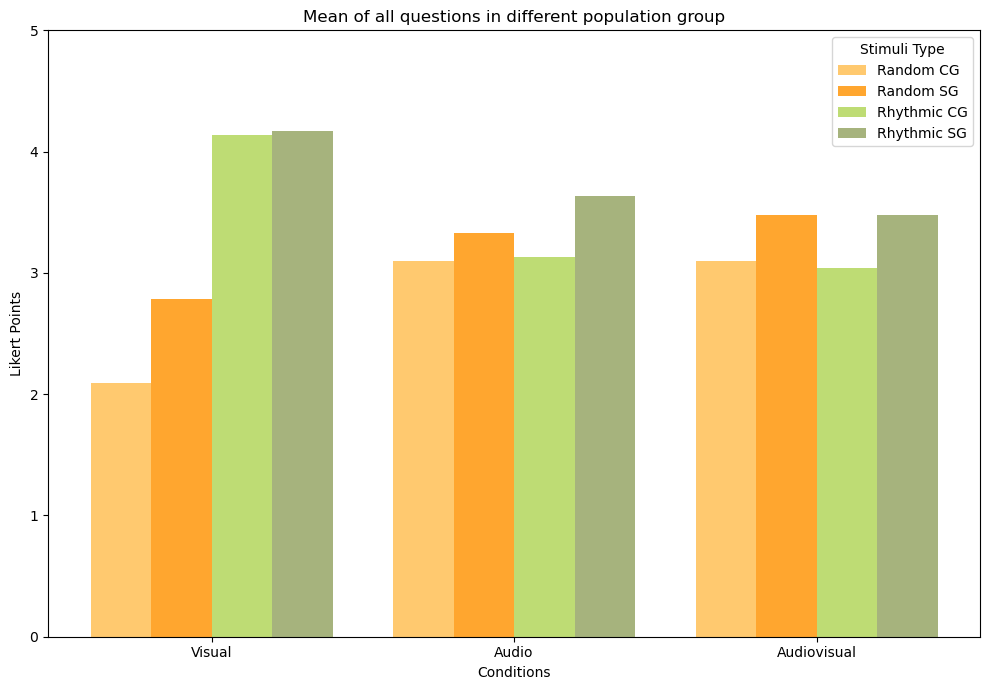
\includegraphics[width=0.85\textwidth]{bar_plots/mean stroke and control.png}
    \caption{Mean of the results of all behavioral question divided by population groups}
    \label{fig: mean_population_condition} 
\end{figure} 
\begin{figure}[H]
    \centering
    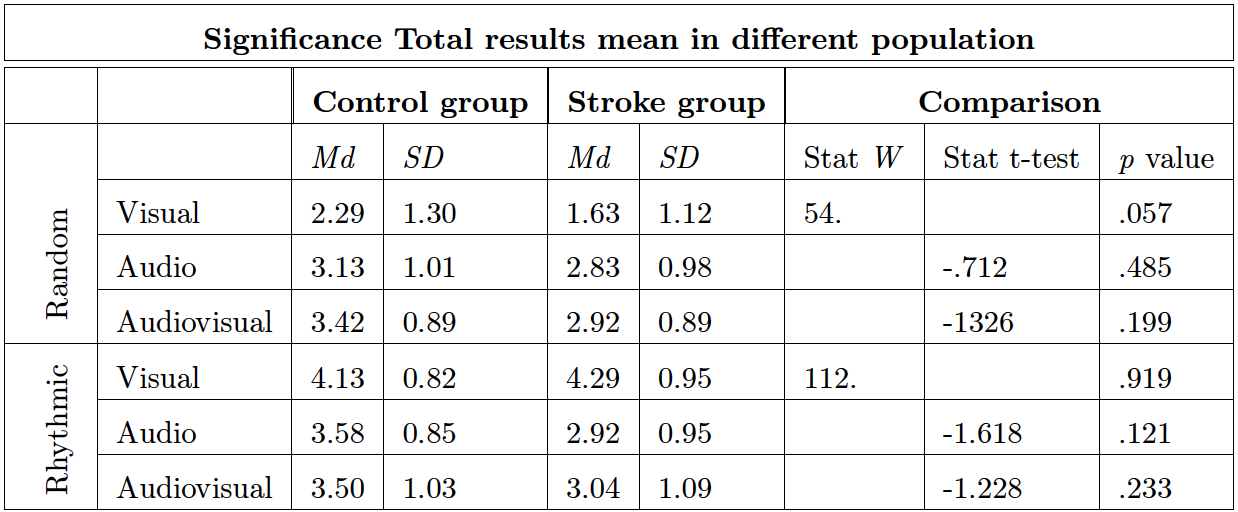
\includegraphics[width=0.70\textwidth]{significance_tables/tot_mean_pop.png}
    \caption{Significance of the results of all behavioral questions, comparing different population groups, using Wilcoxon Signed-Rank Test (\textit{W}) or Paired Samples t-Test (\textit{t})}
    \label{fig: significance_total_mean_pop} 
\end{figure} 

\clearpage
\subsection*{Correlation between physical activity and brain activation}
\begin{figure}[H]
    \centering
    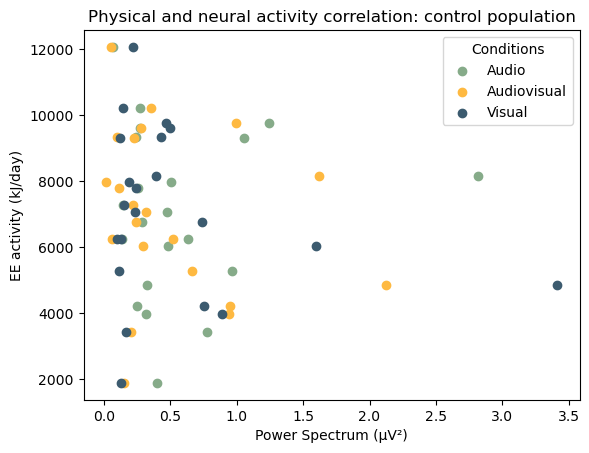
\includegraphics[width=0.75\textwidth]{correlations/correlation_healthy.png}
    \caption{Correlation between activity and neural activation in the control group}
    \label{fig: correlation control} 
\end{figure}
\begin{figure}[H]
    \centering
    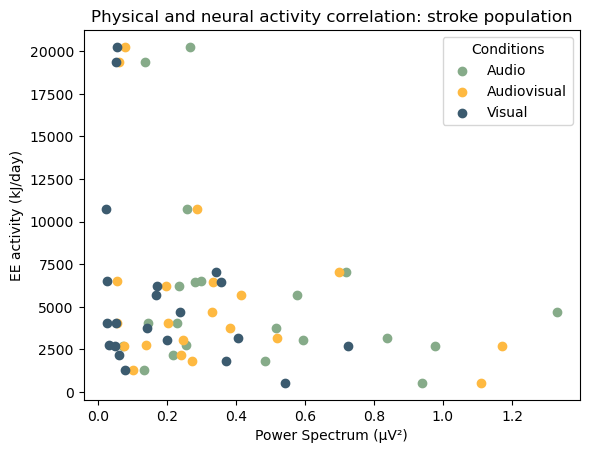
\includegraphics[width=0.75\textwidth]{correlations/correlation_stroke.png}
    \caption{Correlation between activity and neural activation in the stroke population}
    \label{fig: correlation stroke} 
\end{figure}
\begin{figure}[H]
    \centering
    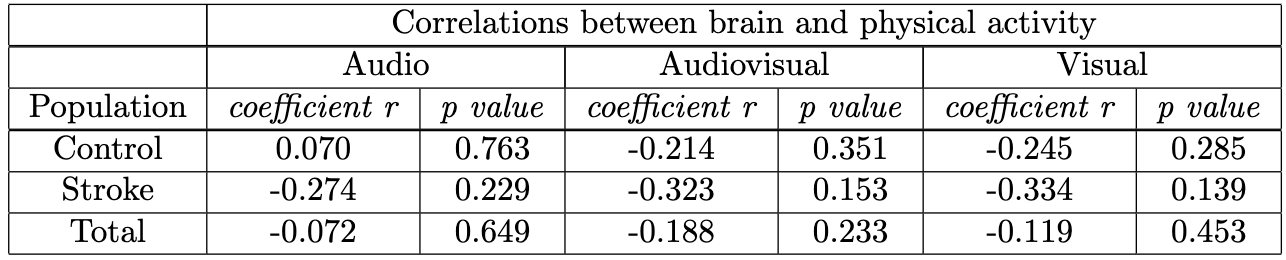
\includegraphics[width=0.75\textwidth]{correlations/corr_values_activeq.png}
    \caption{Correlation values: Pearson correlation coefficient \textit{r} and \textit{p} value}
    \label{fig: correlation values} 
\end{figure}

\clearpage
\subsection*{Correlation between brain activation and behavioral questions}
\begin{figure}[H]
    \centering
    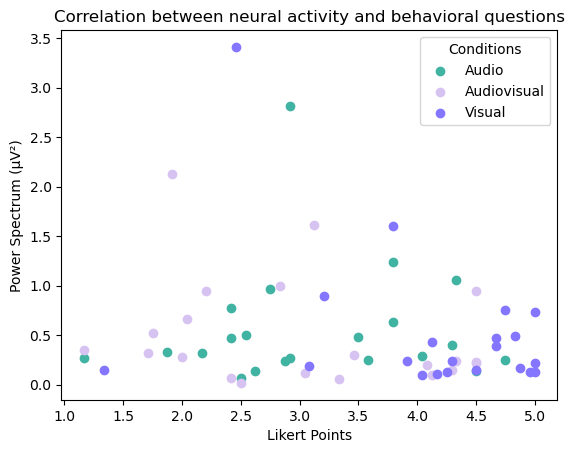
\includegraphics[width=0.75\textwidth]{correlations/corr_na_q_control.png}
    \caption{Correlation between neural activation and behavioral questions in the control group}
    \label{fig: correlation control questions} 
\end{figure}
\begin{figure}[H]
    \centering
    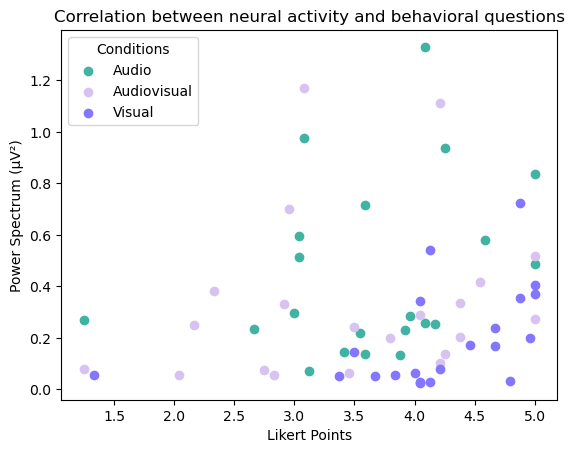
\includegraphics[width=0.75\textwidth]{correlations/corr_na_q_stroke.png}
    \caption{Correlation between neural activation and behavioral questions in the stroke population}
    \label{fig: correlation stroke questions} 
\end{figure}
\begin{figure}[H]
    \centering
    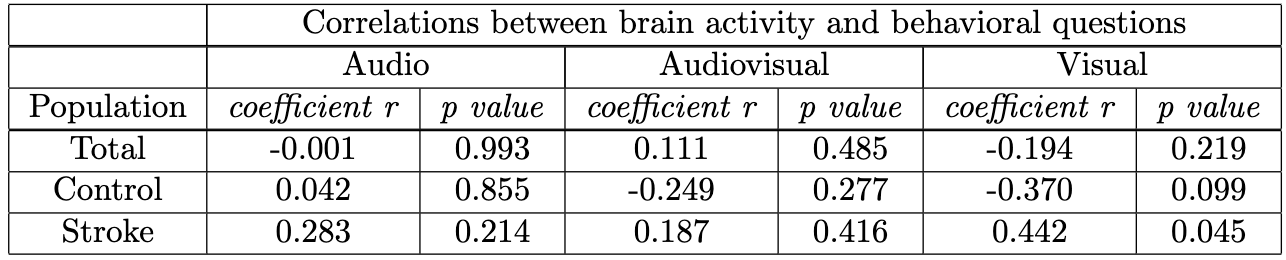
\includegraphics[width=0.75\textwidth]{correlations/corr_values_na_q.png}
    \caption{Correlation values: Pearson correlation coefficient \textit{r} and \textit{p} value}
    \label{fig: correlation values questions} 
\end{figure}